%%%%%%%%%%%%%%%%%%%%%%%%%%%%%%%%%%%%%%%%%%%%%%%%%%%%%%%%%%%%%%%%%%%%%%%%%%%%%%%%
\documentclass[12pt]{article}

\usepackage[authoryear]{natbib}
\usepackage[top=2.5cm,bottom=2.5cm,left=2.5cm,right=2.5cm]{geometry}
\usepackage{color}
\usepackage{chemarr}
\usepackage{amssymb}
\usepackage{graphicx}
\usepackage{textcomp} 
\usepackage[gen]{eurosym}
\usepackage{amsmath}
\usepackage[margin=1.5cm]{caption}
\usepackage{amsmath,mathtools}
\usepackage{subcaption}
\usepackage[normalem]{ulem}
\usepackage{enumitem}
\usepackage{setspace}
\usepackage{nth}
\usepackage{float}
\doublespacing

\usepackage[usenames, dvipsnames]{xcolor}
\colorlet{shadecolor}{gray!5}
\usepackage{listings}
\lstset{ 
	language=bash,                     % the language of the code
	basicstyle=\scriptsize\ttfamily, 	  % the size of the fonts
	numbers=left,                   % where to put the line-numbers
	numberstyle=\tiny\color{Blue},  % the style that is used for the line-numbers
	stepnumber=1,                   % the step between two line-numbers.
	numbersep=5pt,                  % how far the line-numbers are from the code
	backgroundcolor=\color{shadecolor},  % choose the background color.
	showspaces=false,               % show spaces adding particular underscores
	showstringspaces=false,         % underline spaces within strings
	showtabs=false,                 % show tabs within strings adding particular underscores
	frame=tb,                   	  % adds a frame around the code
	rulecolor=\color{Black},        % if not set, the frame-color may be changed on line-breaks within not-black text (e.g. commens (green here))
	tabsize=1,                      % sets default tabsize to 1 spaces
	captionpos=b,                   % sets the caption-position to bottom
	breaklines=true,                % sets automatic line breaking
	breakatwhitespace=false,        % sets if automatic breaks should only happen at whitespace
	keywordstyle=\color{RoyalBlue}, % keyword style
	commentstyle=\color{OliveGreen},% comment style
	stringstyle=\color{ForestGreen} % string literal style
}
%%%%%%%%%%%%%%%%%%%%%%%%%%%%%%%%%%%%%%%%%%%%%%%%%%%%%%%%%%%%%%%%%%%%%%%%%%%%%%%%
\title{\textbf{Thesis Draft}}
\author{Yinrui Li}
\date{}


%\maketitle


\begin{document}
	\maketitle
	%%%%%%%%%%%%%%%%%%%%%%%%%%%%%%%%%%%%%%%%%%%%%%%%%%%%%%%%%%%%%%%%%%%%%%%%%%%%%%%%
	
	
	
	\section{Introduction} 
	Black carbon (BC) is a product of incomplete combustion of fossil fuel, biofuel and biomass burning (Bond et al., 2004; Forsstrom et al., 2013). It strongly absorbs visible light and has been ranked as the 2nd most important individual absorbing agent after CO2, with a climate forcing of +1.1Wm-2 (Bond et al., 2013). Generally, BC aerosols can impact the global atmospheric radiative budget both as atmospheric aerosols, after mixing with other soluble organic materials, or as impurities in snow and ice after being transported to the polar regions and depositing onto their surfaces, resulting in a positive feedback on the surface albedo (Zuberi et al., 2005; Flanner et al., 2007). BC aerosols also have adverse impacts on air quality and human health (Highwood and Kinnersley, 2006).

	Quantifying these impacts requires us to develop faithful model representations of BC burden and its climate-relevant properties such as CCN activities and optical properties. Currently, however, significant discrepancies in model simulated BC remain in most global climate models (GCMs) and large uncertainties of its climate forcing have been shown. For example, previous studies have implied a general overestimation of BC in the mid-upper troposphere in the mid-latitudes, and an underestimation of BC in the lower and middle troposphere at high latitude (Koch et al., 2009; Schwarz et al., 2010; Fan et al., 2012). The simulated BC aerosol absorption optical depth tends to be biased low compared to satellite observations (Koch et al., 2009). These model failures can result from the complex BC aerosol processes and properties that has not been well captured, such as its emissions, coagulation, condensation, dry deposition, wet scavenging, etc. (Hakami et al., 2005; Koch et al., 2009; Shindell et al., 2008). These processes in turn control the evolution of aerosol burden, size distribution, mixing states, and consequently its climate forcing (Schulz et al., 2006; Quaas et al., 2009). 

	Among them, one key process that contributes to the uncertainties and thus needs to be captured is the BC ‘aging’ process, the conversion of freshly emitted, hydrophobic BC to aged, hydrophilic BC through coating with sulfate and organics or coagulation (Langner et al., 1992; Parungo et al., 1994; Liousse et al., 1996). This process directly contributes to the CCN activation and wet removal, and also impacts black carbon’s optical properties by evolving the composition and mixing states of aerosols. Therefore, it plays a significant role in simulating the lifetime of BC, and hence its transport, distributions and climate effects (Croft et al., 2005; Riemer et al., 2004). In addition, previous studies have found that the parameterizations of the aging process can significantly affect model results (Liu et al., 2011).

	Albeit its importance, the treatment of BC aging, however, is usually very simplified in global scale models, either by using fixed timescales or parameterized aging rates for the sake of computational limits. The most simplified bulk scheme assumes fully externally mixed populations and often use a fixed aging timescale (on the order of 1-2 days) for conversion of hydrophobic BC to hydrophilic BC (Cooke and Wilson, 1996). There are also more advanced and complicated schemes such as the modal aerosol model or sectional models, computing mechanic transfer rates by assuming aerosol size distributions and mixing levels (Wilson et al., 2001; Bauer et al., 2008, Huang et al., 2013). 

	The representation of BC aging in the Community Atmosphere Model with Chemistry (CAM-Chem), an atmospheric component of the Community Earth System Model (CESM), uses the latter scheme. It applies a 4-mode version of the modal aerosol model (MAM4), where BC is emitted to the primary carbon mode, and then is aged and transferred to the accumulation mode by condensation of sulfate, ammonia and SOA and by coagulation (Liu et al., 2012; Lamarque et al. 2012). In MAM4, a criterion of 8 monolayers of sulfate is used to compute the aerosol transfer rate from primary carbon mode to accumulation mode. It assumes that BC particle is aged after condensing 8 monolayers of sulfate. However, previous study has shown that considerable sensitivities exist regarding the choices of the number of monolayers and other parameters, and significant model biases in BC burden have been found compared to HIPPO observations (Liu et al., 2015). 

	Furthermore, Laura et al has derived a parameterization that characterizes the aging rates of BC aerosols through gas condensation and particle coagulation from detailed simulations on the particle scale, based on the particle-resolved PartMC-MOSAIC model (Particle Monte Carlo Model for Simulating Aerosol Inter- actions and Chemistry) (Laura et al., 2016). PartMC-MOSAIC is a complex aerosol model that provides detailed information on aging processes at the micro-scale, by tracing the size, composition and mixing states of particles (Riemer et al., 2010). That parameterization can be applied to evaluate and to improve the treatment of BC aging in the global-scale models. 

	In this work, our aim is to assess the representation of BC aerosols in MAM4 of CAMChem model. We conduct several sensitivity runs of BC mixing ratio, mixing states and direct radiative forcing to its condensation criterion, in order to investigate the extent to which those quantities are sensitive to the choices of aging parameters. We also exploit the PartMC-MOSAIC parameterization as the reference to evaluate the performance of MAM4 aging scheme. 

	Our method and model specification are described in Sect.2. Sensitivity analysis of BC is presented in Sect.3. In Sect.4, we focus on process analysis of BC aging by comparing the CAMChem aging timescales with PartMC aging timescales. In Sect.5, we assess the comparability of modeled BC concentration with SP2 measurements. The results are shown in Sect.6. 

	\section{Background}
	
	\subsection{Modal Aerosol Model}
	\subsubsection{Aerosol Dynamic Modeling}
		Aerosols have complex physical processes and a numerical aerosol model can serve as an useful tool to extend our knowledges of aerosol evolution in the atmosphere. Generally, an aerosol model should be able to assemble expressions for the relevant physical processes including coagulation, condensation, nucleation, emission, chemical reaction, etc (Whitby et al., 1991). The approaches to solve those expressions differ by the way that aerosol size distributions are approximated. Some traditional models characterize the particle size distribution as bulk or by single variable such as mass. More complicated models include sectional model that sets discrete size bins and typically assumes species to be internally mixed in each bins and externally mixed between different bins (Jacobson et al., 1997, Adams et al., 1999). This approach neglects the aging process by assuming particles to be internally mixed immediately after emission. Another frequently used representation is called the modal aerosol model (Whitby et al., 1992; Binkowski et al., 1995). Aerosols are viewed as distinct populations of particles that is distinguished by their size or chemical composition, and the size distribution of each population is approximated by some analytical distribution function (Binkowski et al., 1995). Each region of the size distribution is called a mode. The size of the particles in each population is typically approximated by a lognormal distribution characterized by the mean diameter $\mu$ and a standard deviation $\sigma$. The accuracy of the model largely depend on how well the size distribution functions of the modes can represent the actual aerosol size distributions.  
	
		Figure~\ref{fig_P4} shows a typical categorization of 	aerosols by their size distributions. Particles less than 0.1~$\mu$m go into the nucleation mode, particles in the size range 0.1--2~$\mu$m go into the accumulation mode, and particles larger than 2~$\mu$m go into the coarse mode. Similarly, in CAM-chem model, a 3-mode version of modal aerosol model (MAM3) that has only Aitken, accumulation and coarse mode is developed as default, which is efficient for long-term simulations (Liu et al., 2012). There are also a 7-mode version (MAM7) that has Aitken, accumulation, primary carbon, fine dust and fine sea salt, coarse dust and coarse sea salt modes, and a 4-mode version (MAM4) that has an additional primary carbon mode on top of MAM3 for the treatment of the microphysical aging processes of primary carbonaceous aerosols (Liu et al., 2015). 
	\begin{figure}[H] 
		\begin{center}
			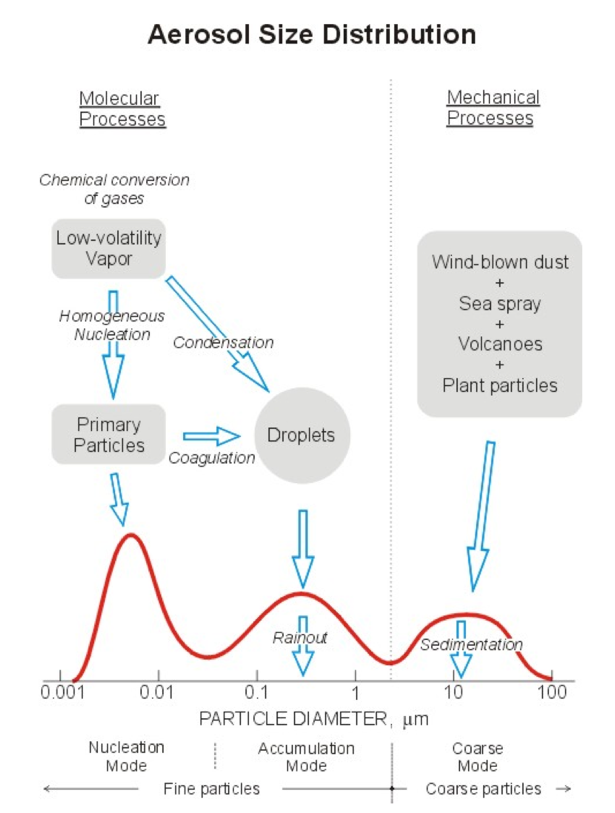
\includegraphics[width = 0.6\textwidth]{Figure04}
			\caption[]{\label{fig_P4} Aerosol Size Distribution. (www.ems.psu.edu/~lno/Meteo437)}
		\end{center}
	\end{figure}
		
	\subsubsection{Moment and Moment Dynamic Equation}
		Modal aerosol model typically assumes lognormal size distributions for each mode (Equation ~\ref{eq:1}) by setting an changeable mean diameter $D_{\rm g}$ and an unchangeable standard deviation $\sigma_{\rm g}$. 
		\begin{align}\label{eq:1}
		n(\text{ln}D) = \frac{N}{\sqrt{\pi}\text{ln}\sigma_{\rm g}}\text{exp}[-\frac{1}{2}(\frac{\text{ln}(D/D_{\rm g})}{\text{ln}\sigma_{\rm g}})^2]
		\end{align}
		During each time step, it simulates the evolution of aerosols by updating the geometric mean diameter $D_{\rm g}$, total number concentration $N$ and standard deviation $\sigma_{\rm g}$ for each mode, solved from their aerosol dynamic differential equations. Those differential equations are designed to catch the physical processes that will drive the evolution of aerosols, such as coagulation, condensation, nucleation, emission, chemical reaction, etc.
	
		 However, while the differential equations for the total number $N$ is easy to obtain, it is hard to find the analogous equations for $D_{\rm g}$ and $\sigma_{\rm g}$. In order to avoid this problem, some kind of integral form called moment is hence introduced to replace the traditional form of differential equations. The mathematical expression of the kth moment is defined as:
	 \begin{align}
	 M_\text{k} = \int_{-\infty}^{+\infty}D^kn(\text{ln}D)d\text{ln}D = ND_{\rm g}^k\text{exp}[\frac{k^2}{2}\text{ln}^2\sigma_{\rm g}]
	 \end{align}
	 \begin{flushleft}
	 	$k = 0$ : total number $N = M_0$ \\
	 	$k = 2$ : total surface area $S = \pi M_2$ \\
	 	$k = 3$ : total volume $V = \frac{\pi}{6}M_3$ \\
	 \end{flushleft}
	, where the total number, surface area and volume of particles in one mode are analogous to the \nth{1} moment, \nth{2} moment and \nth{3} moment respectively. 
	
	The corresponding integral form of dynamic differential equation, called moment dynamic equation, is shown below (Binkowski et al., 1995):
	 \begin{align}
	 \begin{split}
	 \frac{\partial M_\text{k}(t)}{\partial t} = &
	 \underbrace{\nabla \dot M_k}_\text{\clap{convection}} - \underbrace{\nabla \dot \int_{0}^{\infty}D^k\times c(D,t)n(D,t)dD}_\text{\clap{external forces}} \\
	 &+ \underbrace{\nabla \dot \int_{0}^{\infty}D^k\times D(D,t)\nabla n(D,t)dD}_\text{\clap{diffusion}} \\
	 &+ \underbrace{\int_{0}^{\infty}\frac{dD^k}{dV(D)}\times \frac{\partial V(D)}{\partial t}\times n(D,t)dD}_\text{\clap{condensation/evaporation}} \\
	 &+ \underbrace{\int_{0}^{\infty}D^k\times \dot n(D,t)dD}_\text{\clap{nucleation}} \\
	 &+ \underbrace{\frac{1}{2}\int_{0}^{\infty}\int_{0}^{\infty}
	 	(D_{1}^3+D_{2}^3)^{\frac{k}{3}}\times \beta(D_{1},D_2)\times n(D_1, t)\times n(D_2,t) dD_1dD_2}_\text{\clap{coagulation gain}} \\
	 &-\underbrace{\frac{1}{2}\int_{0}^{\infty}\int_{0}^{\infty}
	 	(D_{1}^k+D_{2}^k)\times \beta(D_{1},D_2)\times n(D_1, t)\times n(D_2,t) dD_1dD_2}_\text{\clap{coagulation loss}}
	 \end{split}
	 \end{align}
		The coagulation terms only represent intramodal coagulation here. When there are more than 2 modes, the equation will include more coagulation terms in the same form as the fifth and sixth term, in order to represent intermodal gain and loss due to coagulation.
	
		Generally, modal aerosol model will solve the moment differential equations for $M_0$, $M_3$ and $M_6$, and then derive $N$, $D_{\rm g}$ and $\sigma_{\rm g}$ from the three moments. $M_6$ is chosen because the coagulation term can be integrated analytically. 
	
		In our study, we used a 4-mode version of modal aerosol model (MAM4) of CAM-chem that has aitken mode, accumulation mode, coarse mode and a specially designed primary carbon mode for the treatment of the microphysical aging processes of primary carbonaceous aerosols. More description about MAM4 is in section 3.1. MAM4 assumes that the standard deviation $\sigma_{\rm g}$ for each mode is fixed, whereas $N$ and $D_{\rm g}$ are changeable with time. For each time step the model will solve the dynamic differential equations for $M_0$ and $M_3$, and then derive $N$ and $D_{\rm g}$ from the two moment equations.
	
	\subsection{BC Mixing States in the Arctic}
	\subsubsection{Mixing States and its Importance on Climate}
		Current representation of aerosol and its impact on climate in global models still has large uncertainties, mostly due to the difficulties to capture the microphysical and chemical processes that drive the evolution of aerosol particles in the atmosphere. One factor that may affect aerosol behavior significantly in those processes and also its properties as an climate forcing agent is call the mixing state, the level to which particles are internally or externally mixed with other species or in between. Figure~\ref{fig_P5} shows an observation of the chemical species compositions of single aerosol particles. It is obvious that most aerosols are not pure, and can be mixed with other species. 
		
		Several studies have implied that mixing states affect the climate-related aerosol properties such as optical properties or cloud condensation nuclei activity (Jacobson 2001; Zaveri et al., 2010; Koch et al., 2009). Reddington et al.(2013) found that the model-observation biases in BC properties are much greater than for the overall particle distribution, indicating that the model discrepancies can be largely due to the assumptions about the size and mixing state of the emitted carbonaceous particles. Efforts to improve the representation of aerosol mixing states in both regional and global models have also been made (Jacobson 2002; Riemer et al., 2013; Bauer et al., 2008).
	 
	\begin{figure}[H] 
		\begin{center}
			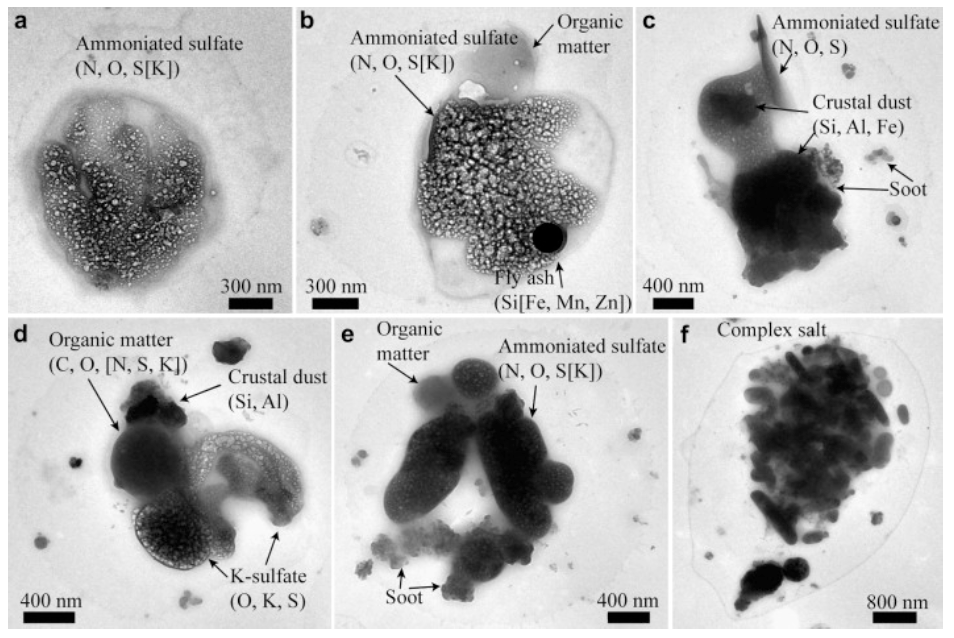
\includegraphics[width = 0.8\textwidth]{Figure05}
			\caption[]{\label{fig_P5} Chemical species compositions of aerosol particles. (Li et al.,2011.)}
		\end{center}
	\end{figure}
	
		\newpage
		Riemer et al (2013) has pointed out that the mixing state of carbonaceous particles depends strongly on the fuel and combustion type. A quantitative metric for mixing state of aerosol population has been developed using a mixing ratio index $\chi$ defined as the ratio of per particle diversity $D_{\alpha}$ to the bulk population diversity $D_{\gamma}$. It ranges from χ = 0 when all particles are fully externally mixed to χ = 1 when all particles are fully internally mixed. The initial mixing state will be further modified in the atmosphere as particles age through coagulation and condensation. Generally, freshly emitted BC particles will are mostly externally mixed, and then will become more internally mixed as a result of its aging process. PartMC-MOASAIC tracks the individual particles and has a more comprehensive representation on particle level compared to global models. Figure~\ref{fig_P6} shows the evolution of mixing states for BC particles as they age in the atmosphere. It is obvious that they become more externally mixed as time goes by. The accuracy of BC mixing state and related climate properties greatly depend on the representation of its aging process in models.
	
	\begin{figure}[H] 
		\begin{center}
			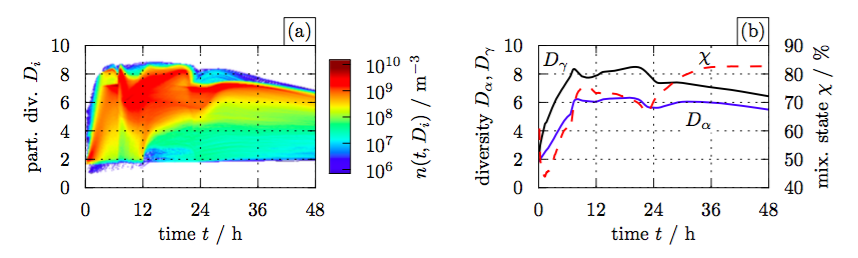
\includegraphics[width = 1\textwidth]{Figure06}
			\caption[]{\label{fig_P6} Diversity and mixing state evolution for BC-containing particles in the urban plume case. (a) Distribution of per-particle diversity $D_{i}$ as a function of time. (b) Time series of average per-particle diversity $D_{\alpha}$, bulk diversity D$D_{\gamma}$, and mixing state index $\chi$ (Riemer et al.,2013.)}
		\end{center}
	\end{figure}
	
		 The mixing states of aerosols have a close effect on its climate properties (CCN properties, optical properties, etc.). In our study, we computed the average population hygroscopicity $\kappa$ as an implication to mixing states for each mode of the 4-mode modal aerosol model (MAM4) in CAM-chem. 
	  
	\subsubsection{BC Mixing States in the Arctic}
	
	
	
	\subsection{Size Range of SP2 Measurements}
		Single particle soot photometer (SP2) quantifies refractory black carbon (rBC) mass by using a laser to heat rBC to evaporation and measuring their emitted thermal radiation (Figure~\ref{fig_P9}). It measures the BC particle cores over a calibrated volume equivalent diameter (VED) range of 55--400~nm. This method is suited for the detection of BC mass in the accumulation mode (Schwarz et al., 2010), but unlikely to represent the total ambient number and mass concentrations of BC particles. The SP2 number-detection efficiency at sea level pressure is reported to be 100$\%$ for BC above 90~nm VED (Schwarz et al., 2010a, Figure~\ref{fig_P8}), so following Reddington et al., 2013, we regarded 90~nm--400~nm as the efficient diameter range.
		
		In order to compare model simulated BC to observations, it is important to first make sure that most of the modeled BC mass is in the size range of SP2 measurements (e.g., in source regions, freshly emitted BC can be smaller than 100~nm). In our study, we estimated the mass fraction of modeled BC in the size range corresponding to SP2 measurement in preparation for further comparison with observations, especially in the Arctic region.
		
		 \begin{figure}[H] 
		 	\begin{center}
		 		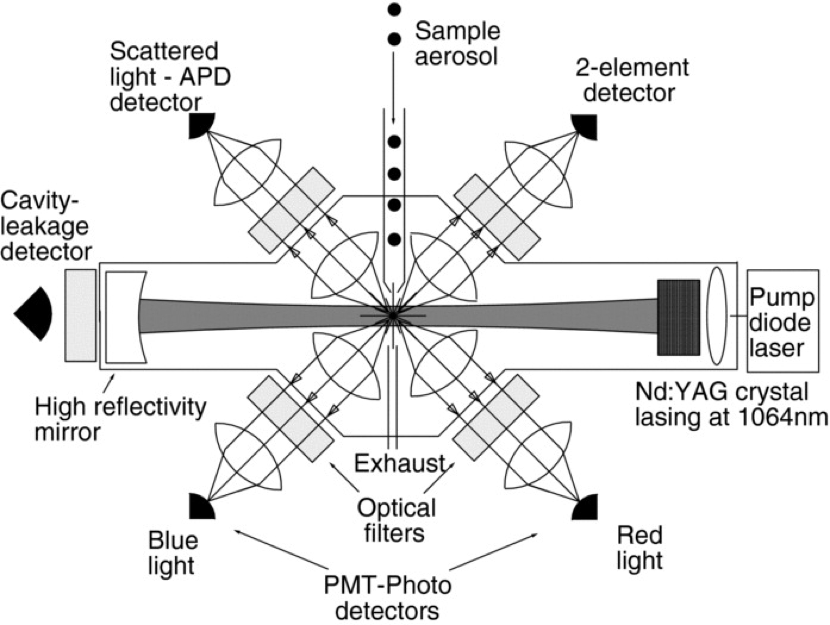
\includegraphics[width = 0.7\textwidth]{Figure09}
		 		\caption[]{\label{fig_P9} Schematic of the Single Particle Soot Photometer (SP2). (Schwarz et al., 2010).}
		 	\end{center}
		 \end{figure}
		 
		 \begin{figure}[H] 
		 	\begin{center}
		 		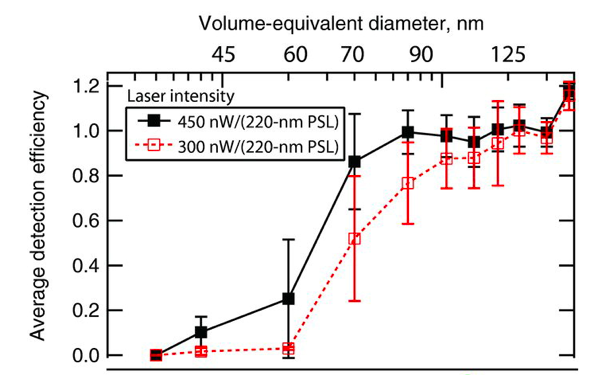
\includegraphics[width = 0.7\textwidth]{Figure08}
		 		\caption[]{\label{fig_P8} The average detection efficiencies in each rBC mass-bin for each laser intensity shown in the legend. Whiskers represent the standard deviation of the values in each mass bin. The top axis shows volume-equivalent diameter (assuming 2 g/cc void-free density for rBC) that corresponds to denuded rBC-core mass on the bottom horizontal scale (Schwarz et al., 2010).}
		 	\end{center}
		 \end{figure}
	
	
	\newpage
	\section{Methodology}

		\subsection{CAM-chem Model Configurations and MAM4}
		
		CAM-chem model is a global 3-D atmospheric component of the NCAR Community Earth System Model (CESM). It consists of the Community Atmosphere Model (CAM) model and chemical mechanism of a fully implemented model for ozone and related chemical tracers (MOZART-4) which includes 191 chemical tracers and over 400 reactions (Tilmes et al., 2016). CAM-chem model can be run either with interactive meteorology coupled to a free-running ocean with specified sea ice and sea surface temperature (free-running configuration), or with specified meteorology which read in winds, air temperature, surface pressure and heat fluxes (offline configuration) (Lamarque et al., 2012). It is also coupled to the land model, involving emissions from biogenic sources by the Model of Emissions and Aerosols from Nature (MEGAN) (Guenther et al., 2012). 

		For our study, we chose the CESM 1-2-2 CAM-chem configured with the offline meteorological data from the Global Earth Observing System (GEOS-5) of the Global Modeling Assimilation Office of NASA, and launched one-year simulation for 2010 with a standard horizontal resolution of 1.9  latitude by 2.5 longitude and a vertical resolution of 56 layers in order to match the resolution of the input meteorology field. We use the Intergovernmental Panel on Climate Change (IPCC) Fifth Assessment report (AR5) gridded POM and BC emissions for the period 1850-2010 in decadal increments (Lamarque et al., 2010). This inventory covers a wide range of sources including anthropogenic emissions (without injection heights) originating from domestic, energy, industry, transportation, waste treatment and ship activity sectors, and natural emissions (elevated) from forest fire and grass fire. It assumes that the POM emissions are higher than the OC emissions by a factor of 1.4 (Liu et al., 2012) and the injection heights for fires are from Dentener et al., 2006. The model treats hydrophobic BC and hydrophilic BC as two separate species, and all the freshly emitted BC falls into the first category. 

		There are three versions of modal representation of aerosol in CAM-chem. A 3-mode version of modal aerosol model (MAM3) that has only Aitken, accumulation and coarse mode is developed as default, which is efficient for long-term simulations (Liu et al., 2012). There are also a 7-mode version (MAM7) that has Aitken, accumulation, primary carbon, fine dust and fine sea salt, coarse dust and coarse sea salt modes, and a 4-mode version (MAM4) that has an additional primary carbon mode on top of MAM3 for the treatment of the microphysical aging processes of primary carbonaceous aerosols (Liu et al., 2015). MAM assumes lognormal size distributions for each mode by setting an unchangeable standard deviation and a changeable mean diameter, and predicts the changes of the size distributions of its particles with time in each mode. In MAM3, all BC particles are assumed to be aged and put directly into the accumulation mode, where particles are exposed to in-cloud and below-cloud wet deposition. In our study, we applied the newly developed MAM4 model, where the freshly emitted BC/POM particles will come directly into the hydrophobic primary carbon mode. The hygroscopicity of BC is set to be 0, and the hygroscopicity of POM is set to be 0.10, allowing them to experience some in-cloud scavenging in the primary carbon mode. After the aging process due to condensation of sulfate aerosols, ammonia and some semi-volatile organic aerosols and inter-mode or intra-mode coagulation, the fresh carbonaceous particles can be transferred from the primary carbon mode to the accumulation mode, viewed as being aged. A schematic of aerosol modes and associated tracers in MAM4 is shown in Figure~\ref{fig_P1}.
		\begin{figure}[H] 
			\begin{center}
				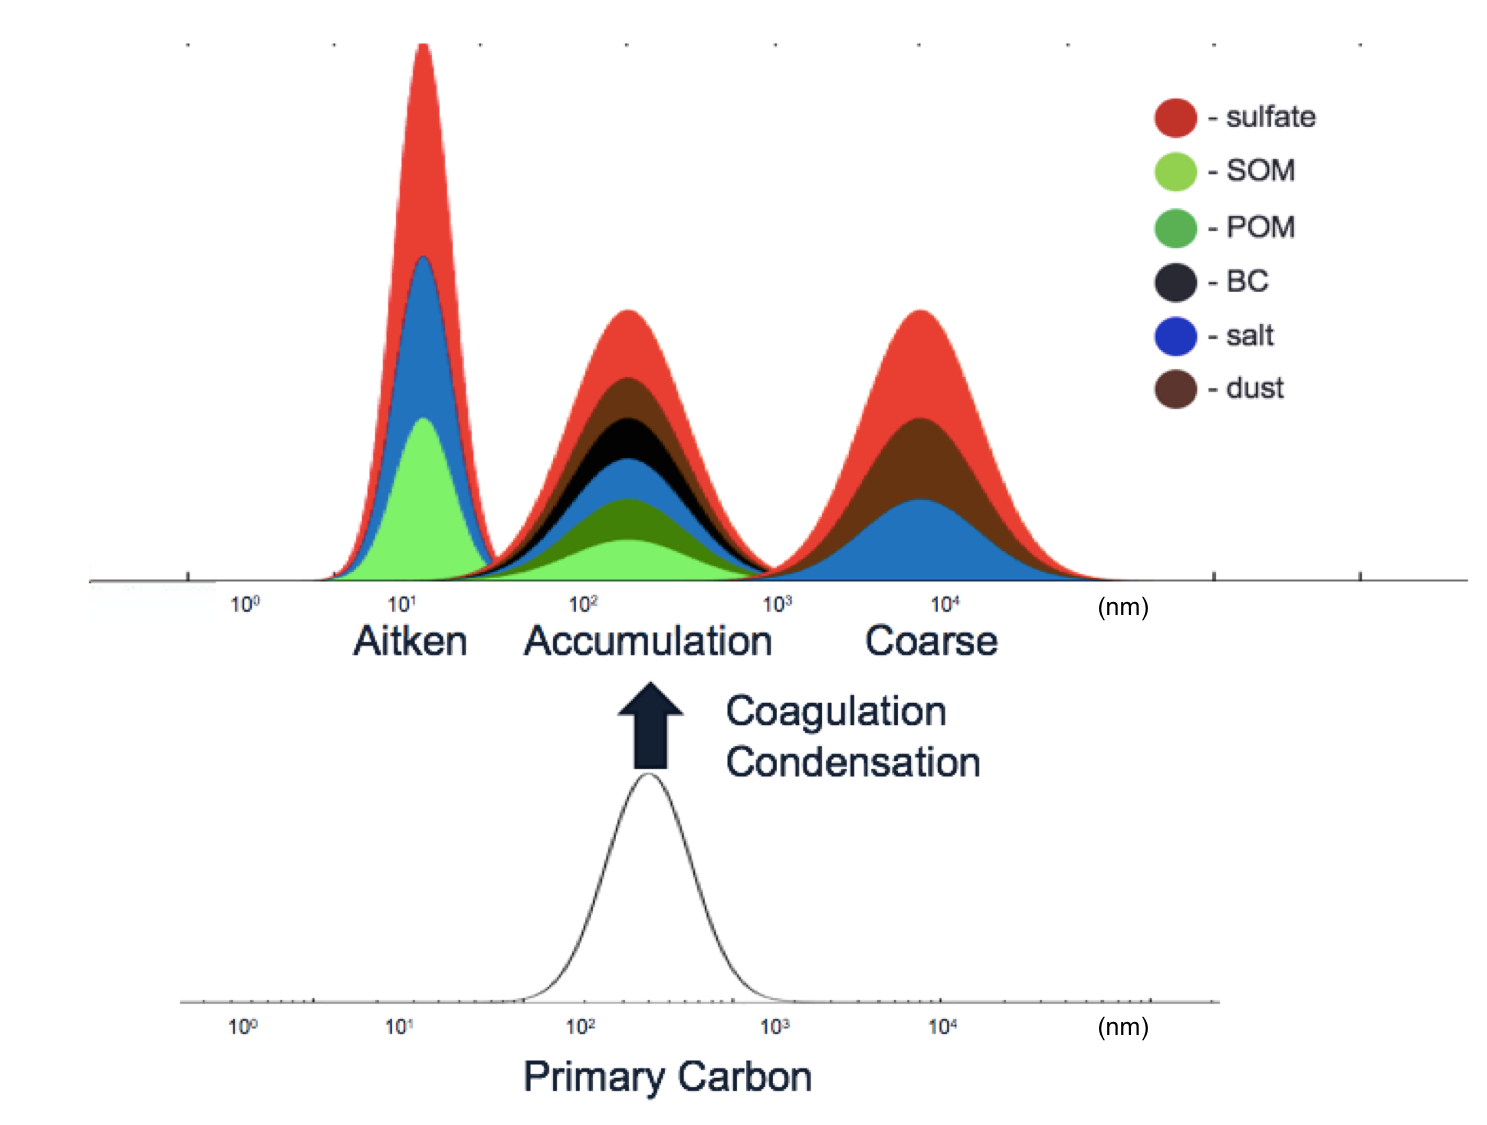
\includegraphics[width = 0.9\textwidth]{Figure01}
				\caption[]{\label{fig_P1} Schematic of aerosol modes and associated tracers in MAM4.}
			\end{center}
		\end{figure}
			
		
		 \subsection{8-monolayer of sulfate Condensation Criterion}
		
		 In MAM4, condensation of sulfate, ammonia and semi-volatile organics to carbonaceous particles are treated in a dynamic way, where a monolayer condensation criterion is applied. It assumes that BC particles become hydrophilic after condensing 8-monolayer of sulfate onto its core surface, and then this mass will be transferred from the primary carbon mode to the accumulation mode based on the standard mass transfer expressions, regarded as being aged (Liu et al., 2012). A schematic of the 8-monolayer condensation criterion is shown in Figure~\ref{fig_P3}. The depth of one monolayer of sulfate is equal to the molecular diameter of sulfate particle ($4.76\times 10^{-10}$~m).
		 \begin{figure}[H] 
		 	\begin{center}
		 		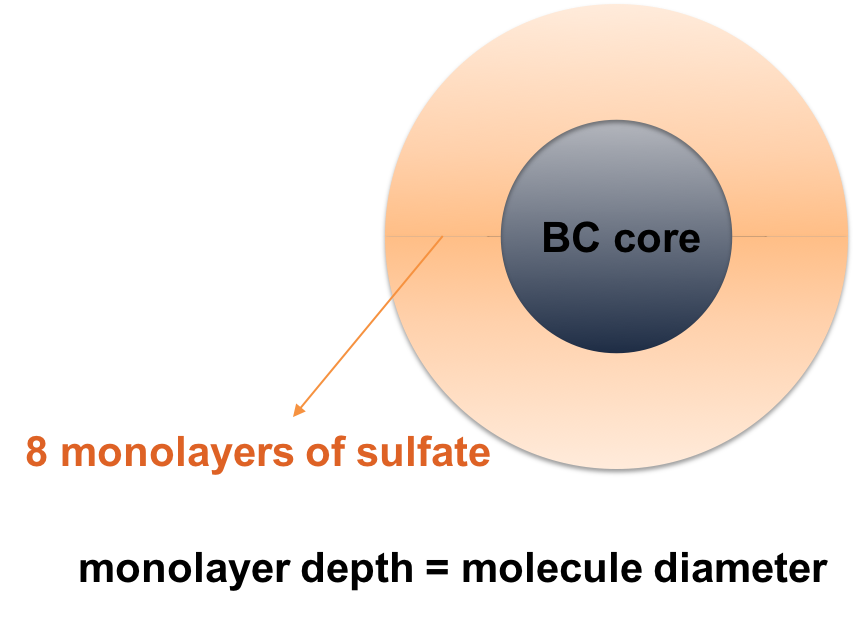
\includegraphics[width = 0.5\textwidth]{Figure03}
		 		\caption[]{\label{fig_P3} Schematic of 8-monolayer of sulfate criterion.}
		 	\end{center}
		 \end{figure}
		 
		 Currently, the condensation of sulfate and ammonia is assumed to be irreversible, whereas the condensation of semi-volatile organics (SOA) is reversible. Sulfate is produced from $\rm{SO}_{2}$ aqueous oxidation in bulk cloud water by ozone and $\rm{H}_{2}\rm{O}_{2}$, based on MOZART treatment (Tie et al., 2001). An accommodation coefficient (0.65), that is the probability of sticking when the gas molecules encounters the surface of an aerosol particle is used for all the three species (Liu et al., 2012). 
		 
		 Generally, for each time-step, the model computes the ratio of the  condensed soluble species mass in the primary carbon to the mass that is required to age all the particles in that mode based on the monolayer criterion. Then it assumes that the same ratio of the POM and BC in the primary carbon mode is transfered to the accumulation mode together with the condensed materials. Here we provide a detailed mathematical explanations of this model representation of the condensation scheme. 
		 
		 For each mode, the rate of gas uptake $F_\text{n}$ ($s^{-1}$) is represented as:
		 \begin{equation}
		 F_\text{n} = \int n(\text{ln}D_{\rm{p}})\times C d(\text{ln}D_\text{p}) ,
		 \end{equation}
		 where $D_\text{p}$ is the diameter of the aerosol particles in that mode, $n(lnD_\text{p})$ is the lognormal size distribution, and $C$ is the gas condensation rate (taking sulfuric acit for example):
		 \begin{align}
		 C = 2\pi \times D_\text{p} \times V_{\rm{diff}} \times F(K_\text{n}, A)\\
		 V_{\rm{diff}} = 0.557 \times 10^4 \times 1.75 \times \frac{T}{P}   
		 \end{align}
		 
		 
		 \begin{flushleft}
		 	$K_\text{n}$ : Knudsen number \\
		 	$A$ : accommodation coefficient \\
		 	$F$ : Fuchs-Sutugin correction factor \\
		 	$V_{\rm{diff}}$ : gas diffusivity for  $\rm{H_2SO_4}$
		 \end{flushleft}
		 The rate of total gas uptake $F_{\rm{sum}}$ is hence estimated by summing up $F_\text{n}$ over all 4 modes, and the fraction of gas mixing ratio going to each mode $f_\text{n}$ is equivalent to the ratio of $F_\text{n}$ to $F_{\rm{sum}}$.
		 \begin{align}
		 F_{\rm{sum}}  &= \sum_{k=1}^4 F_\text{n}          &
		 f_\text{n}          &= \frac{F_\text{n}}{F_{\rm{sum}}} 
		 \end{align}
		 
		 With the above information, the fraction of soluble species condensing on aerosols during $\Delta t$ is derived as $(1 - e^{-\Delta t\times F_{\rm{sum}}})$, and the mass mixing ratio of gas uptake that actually going to mode n during one time-step $\Delta t$ is:
		 \begin{equation}
		 \Delta q_\text{n} = q \times f_\text{n} \times (1 - e^{-\Delta t\times F_ {\rm{sum}}})
		 \end{equation}
	
		 The model computes the fraction of carbonaceous aerosols being aged $f_{\rm{age}}$ as the ratio of the volume of actually condensed materials $V_\text{shell}$ to the volume of soluble species required to age all the particles in the primary carbon mode $V_{\rm{8-mono}}$:
		 \begin{align}
		 \begin{split}
		 V_{\rm{shell}} &=  \Delta q_{\rm{SO_4}, n_{\rm{pc}}} \times V_{\rm{SO_4}} \\
		 &+ \Delta q_{\rm{NH_4}, n_{\rm{pc}}} \times V_{\rm{NH_4}} \\
		 &+ \Delta q_{\rm{SOA}, n_{\rm{pc}}} \times V_{\rm{SOA}} 
		 \end{split}
		 \end{align}
		 
		 \begin{align}
		 \begin{split}
		 V_{\rm{8-mono}} = (\pi M_2/ \frac{\pi}{6}M_3) \times d_{\rm{8-mono}}
		 \end{split}
		 \end{align}
		 
		 \begin{align}
		 f_{\rm{age}} &= \frac{V_{\rm{shell}}}{V_{\rm{8-mono}}}  
		 \end{align}
		 
		 \begin{flushleft}
		 	$V_{\rm{SO_4}}$, $V_{\rm{NH_4}}$, $V_{\rm{SOA}}$: factors that convert the unit of mixing ratio to $m^3/$kmol air. \\
		 	$V_{\rm{8-mono}}$: the volume of sulfate required to age all BC particles. \\
		 	$V_{\rm{core}}$: the volume of pure BC. \\
		 	$M_2$ $M_3$: second and third moment of  moment dynamic equation, $\pi M_2/ \frac{\pi}{6}M_3$ is the ratio of aerosol surface area to volume. \\
		 	$d_{\rm{8-mono}}$: the thickness of 8 monolayers of sulfate.
		 \end{flushleft}
		 
		 The mass transfer over $\Delta t$ is then represented as:
		 \begin{align}
		 \Delta q_{n_{\rm{pc}}} &= \Delta q_{n_{\rm{pc}}} - f_{\rm{age}} \times q_{n_{\rm{pc}}}  &&\text{primary carbon mode} \\
		 \Delta q_{n_{\rm{accu}}} &= \Delta q_{n_{\rm{accu}}} + f_{\rm{age}} \times q_{\rm{n_{\rm{pc}}}}  &&\text{accumulation mode}
		 \end{align}
		 
		 
		 \subsection{CAM-chem Aging Timescale}
		 In a first-order aging model, the transition of BC mass from fresh to aged mode can be represented by an aging timescale. The model is given by
		 \begin{align}
		 \frac{dM_{\rm{fresh}}}{dt} = -\frac{1}{t_{\rm{aging}}}M_{\rm{fresh}} 
		 \end{align}
		 $M_{\rm{fresh}}$ is the mass of fresh particles.
		 The aging timescales can represented as the production of the inverse of the mass transfer rate and fresh BC mass. 
		 \begin{align}\label{eq:9}
		 t_{\rm{aging}} = M_{\rm{fresh}}/(-\frac{dM_{\rm{fresh}}}{dt})
		 \end{align}
		 Any particle transition from the fresh to aged mode during a time step is either by coagulation with other particles or by accumulating a certain amount of condensible materials. So the overall aging timescale $t_{\rm{aging}}$ can be represented as the combination of the aging timescales by condensation $t_{\rm{cond}}$ and by coagulation $t_{\rm{coag}}$.
		 \begin{align}\label{eq:10}
		 \frac{1}{t_{\rm{aging}}} =\frac{1}{t_{\rm{coag}}} + \frac{1}{t_{\rm{cond}}}
		 \end{align}
		 Each of the component aging timescales $t_{\rm{cond}}$ and $t_{\rm{coag}}$ can be derived from the corresponding mass transfer rate by applying Equation~ \ref{eq:9}. 
		 
		 In CAM-chem model, BC particles are transfered from the fresh, primary carbon model to the aged, accumulation mode according to mass transfer rates computed from the coagulation and condensation processes respectively. We extracted the mass transfer rates every 6 hours and apply Equation~\ref{eq:9} and Equation~\ref{eq:10} to get the corresponding timescales for aging. We would be able to evaluate the contribution of condensation and coagulation to the overall aging by showing their  timescales separately. In this study, we evaluated the monthly and annually averaged aging timescales. 
		 
		 \subsection{PartMC-MOSAIC Aging Timescale}
		 PartMC-MOSAIC (particle resolved model) can track the evolution of individual particles as they evolve through condensation, coagulation, emission and evaporation of SOA (Fierce et al., 2016). In current version of PartMC, the particles is not tracked individually but is instead assumed to be completely mixed. Previous study has investigated reduced representation of mixing state for simulating aerosol effects on climate (Fierce et al., 2016). It was discovered that using a detailed benchmarking model to simulate gas condensation and particle coagulation can represent simple mixing state sufficiently for modeling cloud condensation nuclei concentrations, and the mixing timescales that characterized this transformation have been parameterized. In our study, we applied that aging timescale parameterization to our global models outputs to evaluate the accuracy of our global model aging timescales.
		 
		Fierce et al applied a series of 100 sensitivity scenarios sampled using Latin hypercube sampling (McKay et al., 1979). Twenty-eight input parameters were applied to represent a range of atmospheric conditions, from highly polluted cases with consequently rapid aging to remote regions with slow aging. Those parameters include environmental variables, aerosol characteristics, aerosol type and gas emissions. In each scenario, they simulate the evolution of carbonaceous particles that is emitted into a population of background aerosol. No new fresh particle will be emitted during this process after the simulation starts, in order the isolate the effects of aging (Laura et al., 2016). The normalized error in the number concentration of CCN computed using the particle-resolved composition and the reduced representation of composition is given by:
		\begin{align}\label{eq:11}
		e_{\rm CCN}(t) = \frac{\int_{0}^{\infty}( \tilde{N}_{\rm CCN}(t,s) - 
			N_{\rm CCN} (t,s))ds}{\int_{0}^{\infty} \tilde{N}_{\rm CCN, q}(t,s)ds}
		\end{align}
		where $\tilde{N}_{\rm CCN}$ is the number concentration of CCN using the reduced composition and $N_{\rm CCN}$ is the CCN using the particle-resolved composition. This error decreases exponentially with time and a regression result has shown a high R-squared value as 93$\%$. The equation can be expressed as:
		\begin{align}
		e_{\rm CCN}(t) = e_{\rm CCN}(t_{0})\text{exp}(-\int_{t_{0}}^{t}\frac{1}{\tau_{\rm mix}(t)} dt) 
		\end{align}
		where $\tau_{\rm mix}$ is the overall aging timescale. 
		A particle is either aged by condensation or by coagulation, so the two processes can be treated as separate process and has their own timescale (Laura et al., 2015). Accordingly, the overall timescale is found to be a function of the condensation growth rate $I(t)$ and the particle number concentration $N(t)$.
		So a more specified parameterization of $\tau_{\rm mix}$ can be derived by regression of the error on $I(t)$ and $N(t)$:
		\begin{align}
		e_{\rm CCN}(t) = e_{\rm CCN}(t_{0})\text{exp}(-k_{\rm cond}\int_{t_{0}}^{t} I(t) dt)\text{exp}(-k_{\rm coag}\int_{t_{0}}^{t}N(t) dt) 
		\end{align}
		Figure~\ref{fig_P2} is an example of determining $k_{\rm coag}$ after setting $I(t)$ to be 0. 
		
		In our study, we computed the number concentration $N$ as the sum of the particle number concentration of all modes, and the condensation growth rate $I$ as the volume condensation rate over the total aerosol surface area. As is mentioned in 3.2, the condensation of SOA is reversible, so the total condensation rate can be positive or negative. Since all fresh BC particles are in the primary carbon mode, we computed the condensation growth rate using the volume condensation rate and surface area extracted from the primary carbon mode. The PartMC-MOSAIC parameterized aging timescales can then be represented as:
		\begin{align}
		\tau_{\rm overall} \approx (k_{\rm cond}I_{\rm cond} + k_{\rm coag}N)^{-1}
		\end{align}
		
		Fierce et al (2016) has shown the estimated e-folding time $\tau_{\rm overall}$ computed from the approximate range of condensation growth rate and number concentration for specific locations (Figure~\ref{fig_P7}). This range can also be used an a reference for global models.
		
		\begin{figure}[H] 
			\begin{center}
				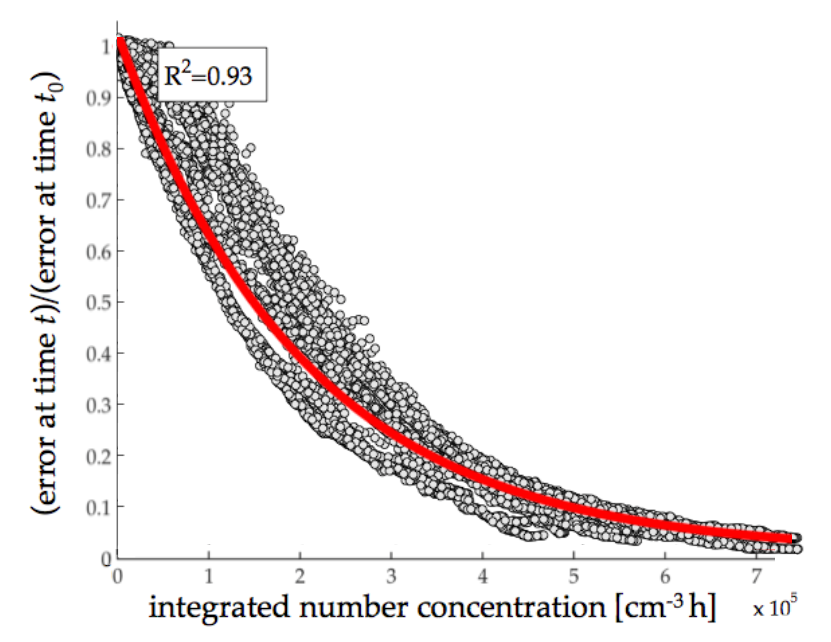
\includegraphics[width = 0.6\textwidth]{Figure02}
				\caption[]{\label{fig_P2}Raw data that is used to construct the regression function (grey dots) and the resulting regression function (black line) for simulations including only coagulation, without condensation (Fierce et al., 2016).}
			\end{center}
		\end{figure}
		
		\begin{figure}[H] 
			\begin{center}
				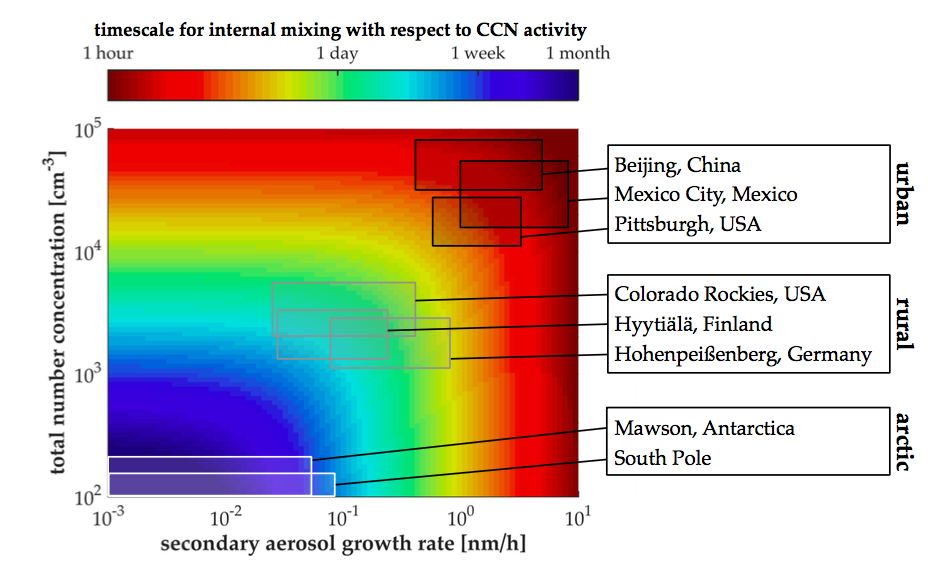
\includegraphics[width = 0.8\textwidth]{Figure07}
				\caption[]{\label{fig_P7}Estimated e-folding time for the error in CCN activity from the internal mixture approximation. (Fierce et al., 2016).}
			\end{center}
		\end{figure}
 
 	\clearpage
 	
	\section{Results}
	\subsection{BC Emissions}
		We use the Intergovernmental Panel on Climate Change (IPCC) Fifth Assessment report (AR5) gridded POM and BC emissions for the period 1850-2010 in decadal increments (Lamarque et al., 2010). Sources include anthropogenic emissions originating from domestic, energy, industry, transportation, waste treatment and ship activity sectors, and natural emissions (elevated) from forest fire and grass fire. The distribution of anthropogenic BC emissions (Figure~\ref{fig_P11}) shows ocean going ship tracks in the Arctic region, and the relatively high emission fluxes in Europe might also be a regional contribution to the BC burden in the Arctic. BC burdens are maximum in industrial regions such as Southeast Asia and biomass burning regions such as Southern Africa and Amazon rainforest. A strong seasonal variation in natural BC emissions can be observed (Figure~\ref{fig_P12}), where the fluxes in September are more than 1000 times higher than the fluxes in March for regions like Amazon rainforest and South Africa, and 10 times higher for the red-colored regions (see left-bottom panel in Figure~\ref{fig_P12}) throughout Russia and Europe. 
		
		\begin{figure}[H] 
			\begin{center}
				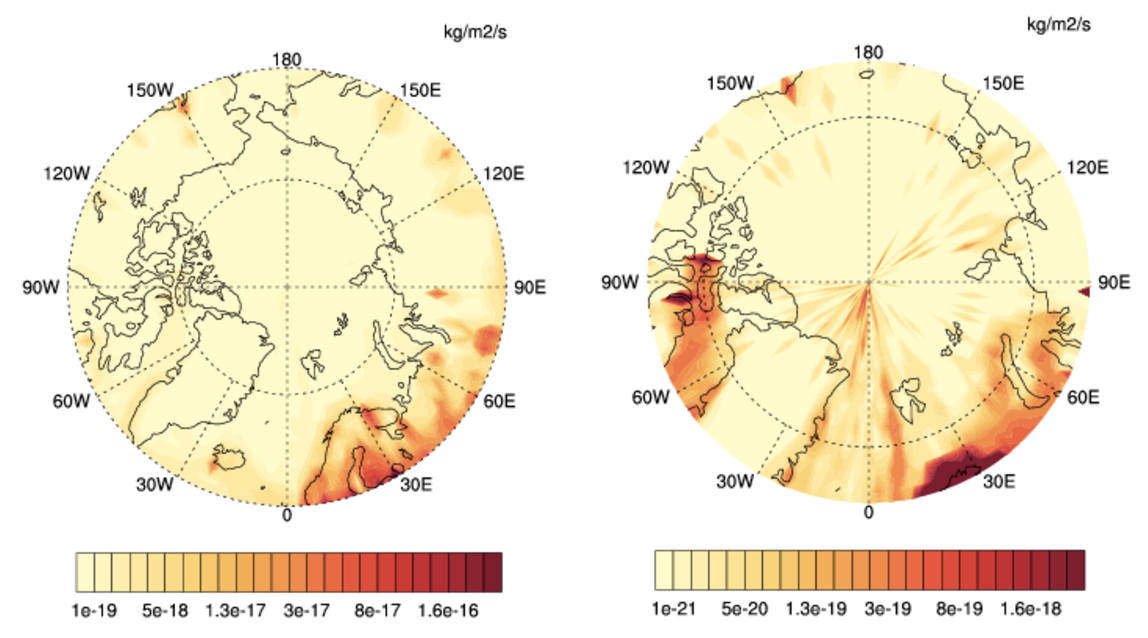
\includegraphics[width = 0.8\textwidth]{Figure11}
				\caption[]{\label{fig_P11} Annual mean anthropogenic emissions of BC emitted at the surface for the year 2010 for 60--90~$^\circ$N (left) and 70--90~$^\circ$N (right).}
			\end{center}
		\end{figure}
		\begin{figure}[H] 
			\begin{center}
				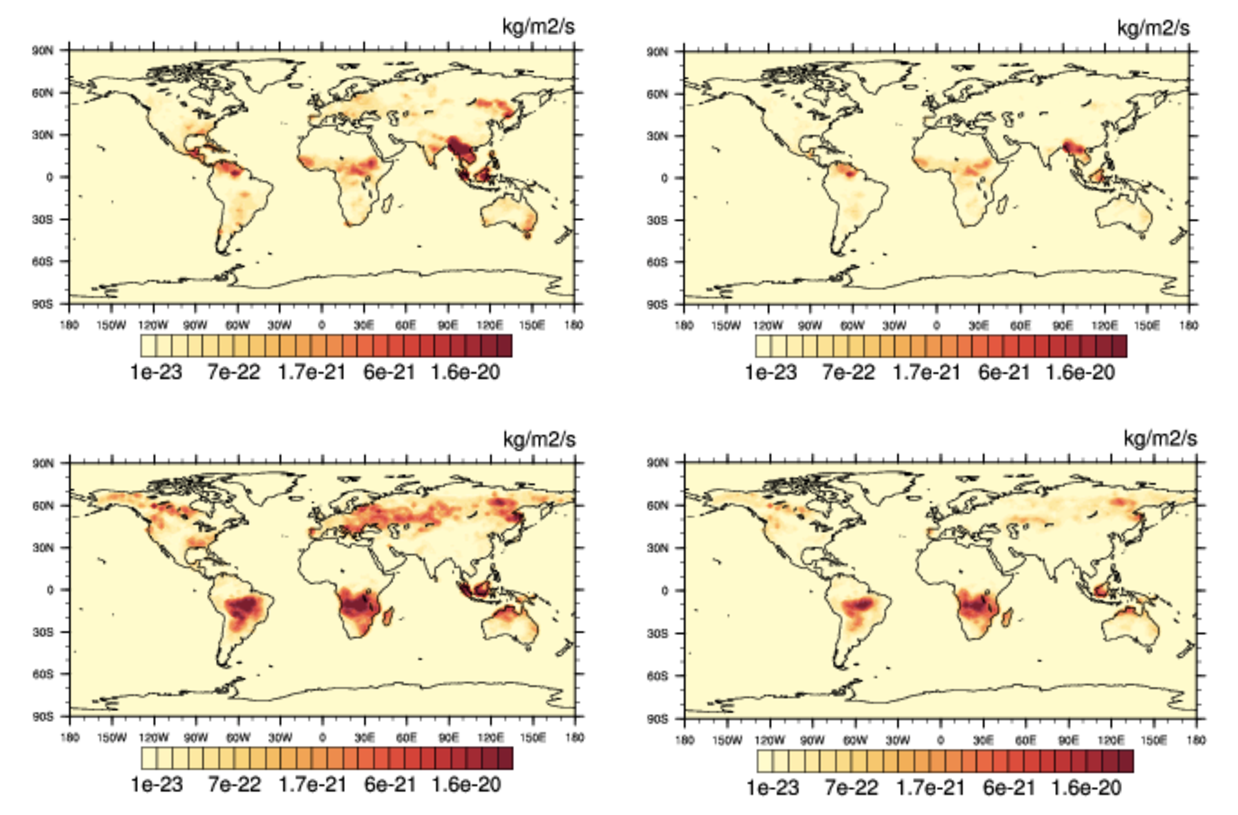
\includegraphics[width = 0.9\textwidth]{Figure12}
				\caption[]{\label{fig_P12} Monthly mean forest fire and grass fire fluxes of BC for March (top panels) and September (bottom panels), at heights of 0--126~m (left panels) and 278--454~m (right panles).}
			\end{center}
		\end{figure}
		
	
	\subsection{Sensitivity on the Number of Monolayers}{\label{sec_1}}
	To explore the model sensitivity to the number of monolayer of sulfate condensation criterion, we conducted four experiments at $1.9^\circ \times 2.5^\circ$ from January 1 2010 to December 31 2010 with offline meteorology, and set the number of mono-layers to 1, 2, 4 and 8 (default) respectively, represented as L1, L2, L4 and L8.	For a larger number of monolayers criterion, more coating material is required to transfer the carbonaceous aerosols from the primary carbon mode to the accumulation mode, hence BC will stay longer in the primary carbon mode and the aging rates will be slower.
	\subsubsection{Horizontal Profiles of BC burdens}
	Figure~\ref{fig_P13} shows the horizontal distributions of BC mixing ratio near the surface in the L8 case (top panel), and the relative differences between L1 and L8 cases (bottom panel), denoted by (L1 - L8)/L8. Generally, BC concentrations in the L1 case are lower than L8 case throughout the globe, because the aging is faster with a smaller threshold of the number of monolayers, and hence more fresh BC will be transfered to accumulation mode. The accumulation mode aerosols are then subject to wet removal, which will prevent them from traveling to remote regions.     
	
	We observed that the relative differences increase along the pathway of BC as it is transported away from the source regions, such as the South Atlantic Ocean downwind of South Africa or the North Pacific near Southeast Asia, both show higher differences than their surrounding regions and can be matched to obvious BC burden gradient along BC pathways over the ocean. Simulated BC burden is most sensitive to the choices of aging criterion in the high-latitude regions where the background concentrations are low, with maximum differences in the annually averaged BC mixing ratio of 16$\%$ near the surface. 
	
	\begin{figure}[H] 
		\begin{center}
			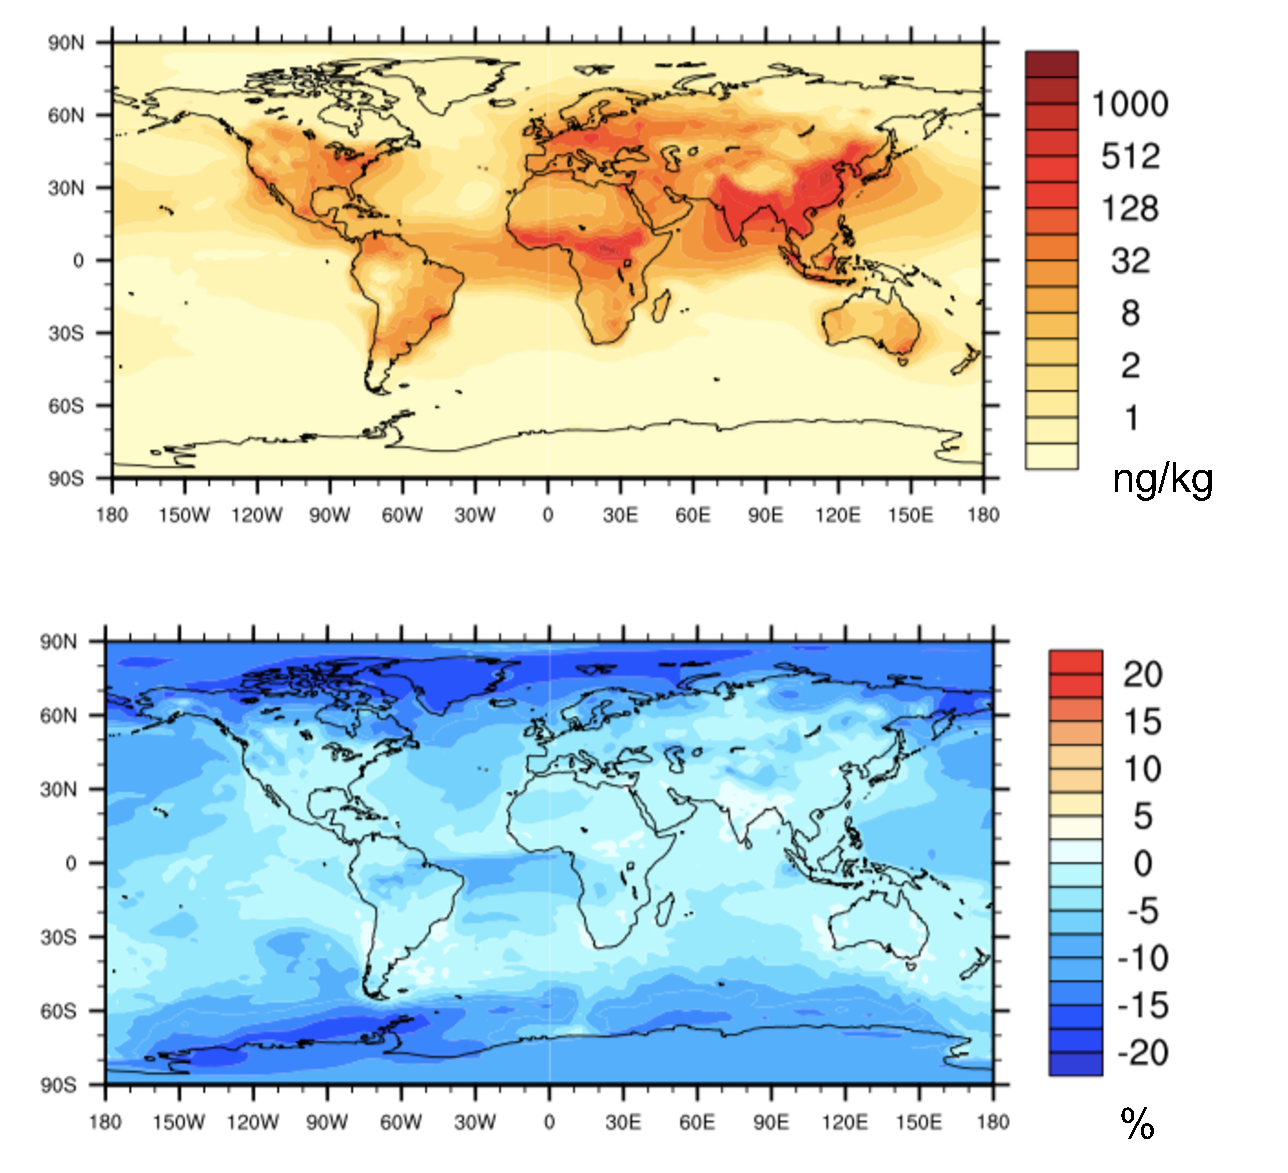
\includegraphics[width = 0.6\textwidth]{Figure13}
			\caption[]{\label{fig_P13} Annual BC mass mixing ratio (top) and relative differences denoted by (L1 - L8)/L8 (bottom).}
		\end{center}
	\end{figure}
	
	\subsubsection{Vertical Profiles of BC burdens}
	Figure~\ref{fig_P14} and \ref{fig_P16} show the sensitivity of BC vertical distributions to the number of monolayers in six regions (Figure~\ref{fig_P15}). Region 1 and 2 are distant from emission sources while the other four regions are dominated either by biomass burning activities (region 3 and 4) or by emissions from both anthropogenic and biomass burning activities (region 5 and 6). It's obvious that BC distributions in distant regions are more sensitive to the number of monolayers (region 1 and 2 compared to 3--6). The maximum relative differences among the six regions are found at 400 hPa in region 2 during March, indicating that the highest model sensitivity can appear at high altitudes near the Arctic. Throughout the source regions, a decreasing trend of BC burdens with height is shown whereas an increasing trend is observed instead for distant regions, probably due to the wet removal process that prevents lower level BC from being transported far away from its sources. These results are still to be further evaluated in the future, considering that the model simulations tend to overestimate BC burdens in the upper troposphere and underestimate BC burdens at altitudes below 400 hPa (Liu et al., 2015). 
	
	Figure~\ref{fig_P14} and \ref{fig_P16} also compare the model simulated BC vertical profiles in March and September in order to explore their seasonal variability. Regions dominated by biomass burning have significant increases of BC burdens in September by 10 order of magnitude (region 3 and 4). BC concentrations tend to be maximum in September because of South American and Africa biomass burning activities in the dry season (Liu et al., 2015). The poleward transport can also be seen from the vertical profile of region 1 at high altitudes above 400~hPa, especially for September. The differences among the four MAM4 experiments are smaller in September especially in the Arctic and oceanic regions. In addition, more BC are concentrated in the upper troposphere in September, probably because of the biomass burning activities produces BC at higher altitudes compared to other sources. 
	
	\begin{figure}[H] 
		\begin{center}
			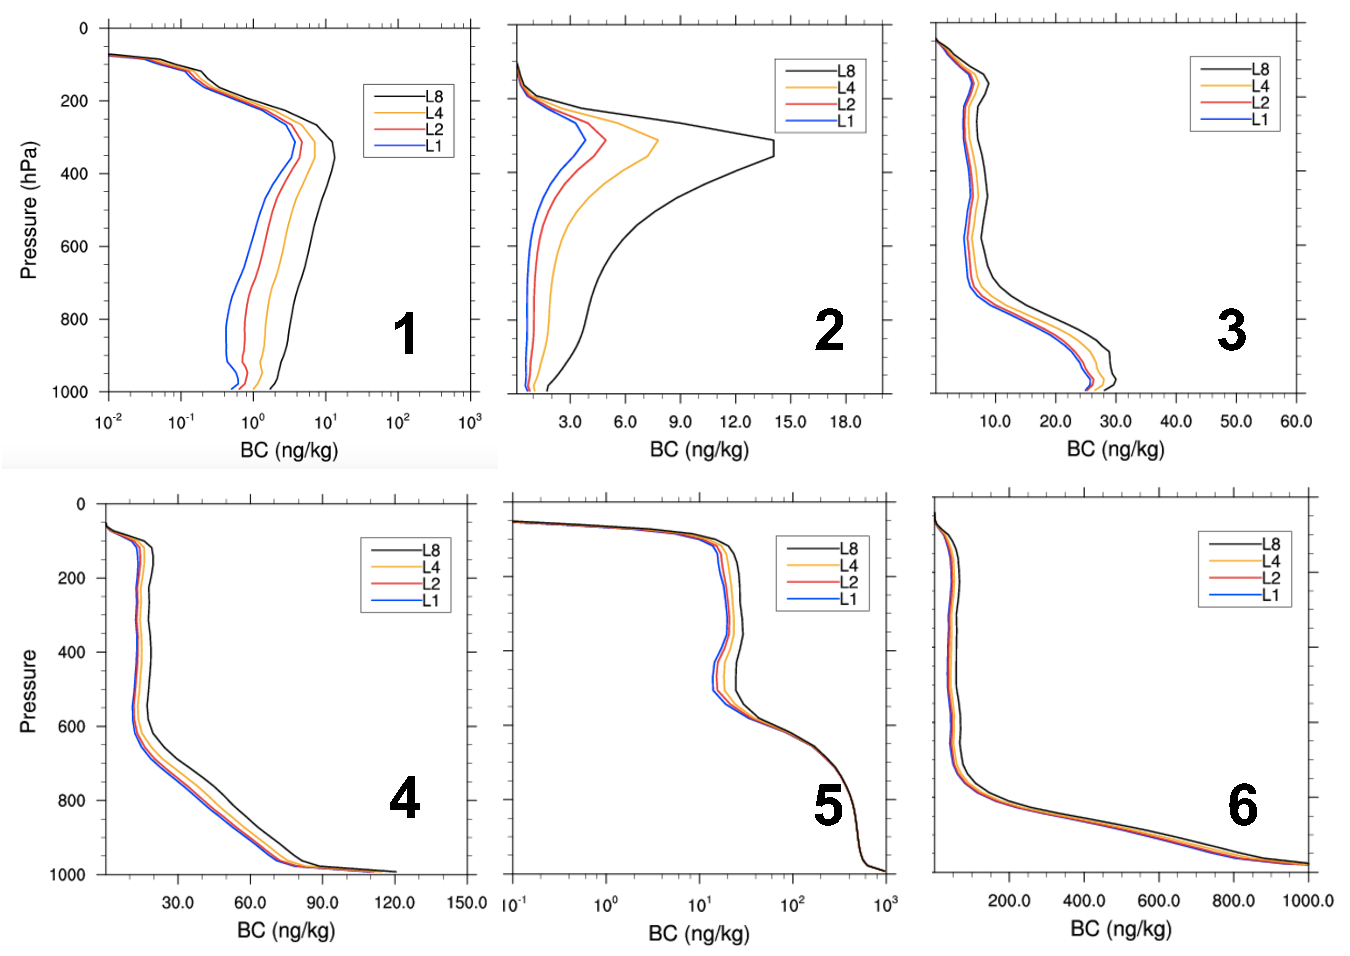
\includegraphics[width = 0.7\textwidth]{Figure14}
			\caption[]{\label{fig_P14} Vertical profiles of mean  burdens for six regions corresponding to Figure~\ref{fig_P15} in March, 2010.}
		\end{center}
	\end{figure}
	
	
	\begin{figure}[H] 
		\begin{center}
			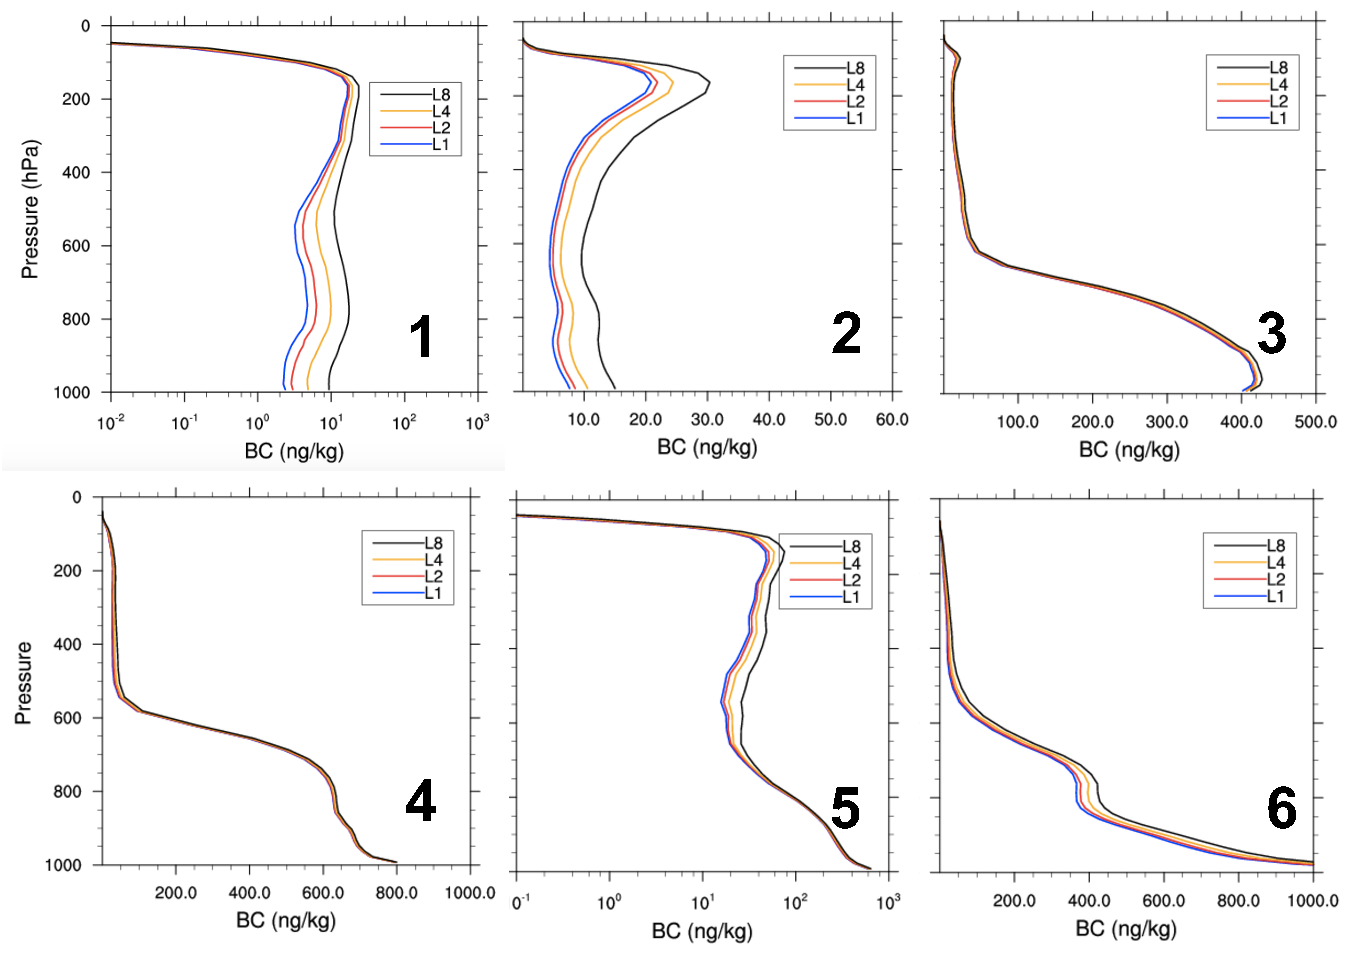
\includegraphics[width = 0.7\textwidth]{Figure16}
			\caption[]{\label{fig_P16} Vertical profiles of mean BC burdens for six regions corresponding to Figure~\ref{fig_P15} in September, 2010.}
		\end{center}
	\end{figure}
	
	\begin{figure}[H] 
		\begin{center}
			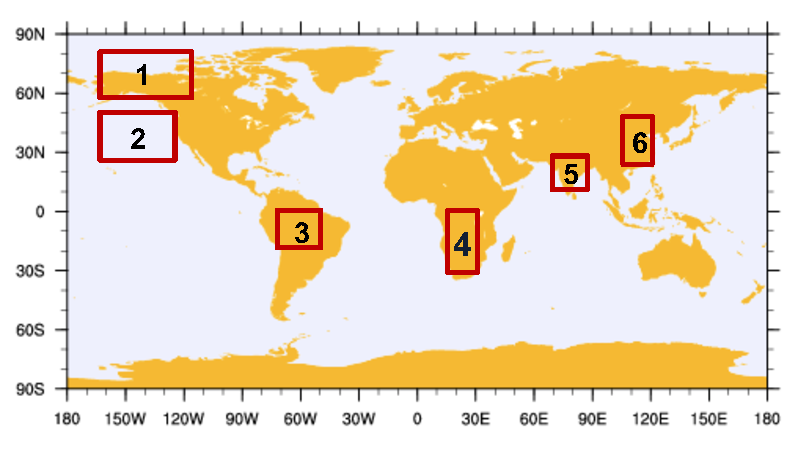
\includegraphics[width = 0.5\textwidth]{Figure15}
			\caption[]{\label{fig_P15} Horizontal map of six regions: Region 1 (162$^\circ$W--112$^\circ$W, 60$^\circ$N--80$^\circ$N), Region 2 (160$^\circ$W--130$^\circ$W, 30$^\circ$N--50$^\circ$N), Region 3 (75$^\circ$W--55$^\circ$W, 10$^\circ$S--1$^\circ$N), Region 4 (15$^\circ$E--30$^\circ$E, 30$^\circ$S--0$^\circ$N), Region 5 (73$^\circ$E--83$^\circ$E, 15$^\circ$N--27$^\circ$N), Region 6 (108$^\circ$E--120$^\circ$E, 23$^\circ$N--43$^\circ$N).}
		\end{center}
	\end{figure}
	
	Figure~\ref{fig_P20} shows the horizontal plots of regional BC concentrations at 859~hPa for the arctic region. The patterns of BC distributions in the two MAM4 experiments are quite different, in addition to their regional mean differences among the cases that has been explained in the previous paragraphs. This finding indicates that the sensitivity of not only the magnitude of BC burdens, but also their latitudinal and longitudinal patterns are both very sensitive to the aging criterion, especially in the middle and upper troposphere. So understanding the BC aging process so as to improve the reliability of the number-of-monolayer criterion is quite important for the accuracy of CAM-chem MAM4 BC simulations.
	
	
		\begin{figure}[H] 
			\begin{center}
				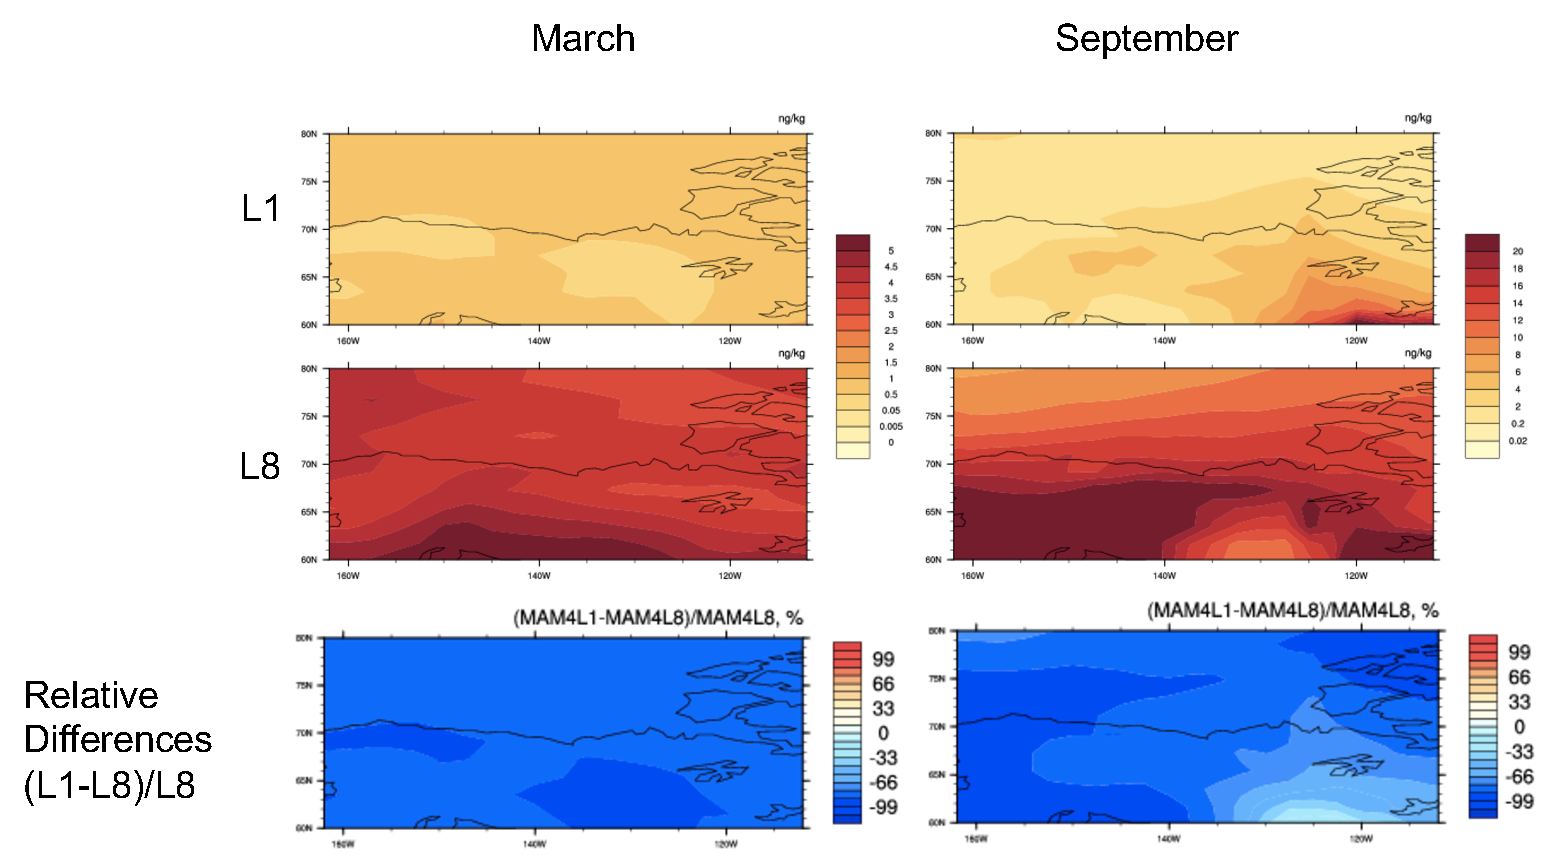
\includegraphics[width = 1\textwidth]{Figure20}
				\caption[]{\label{fig_P20} Horizontal plots of regional BC concentrations at 859~hPa covering region 1 in case L1 (top) and L8 (middle), and the relative differences (bottom) denoted by (L1 - L8)/L8.}
			\end{center}
		\end{figure}

	\subsubsection{BC Deposition Flux}
	We also explored the sensitivity of BC deposition flux through both wet and dry processes to the aging criterions, and compared their differences between two cases (L1 v.s. L8). Figure~\ref{fig_P17} and \ref{fig_P18} shows the relative differences of the monthly averaged wet deposition rates and dry deposition rates respectively, and compares the seasonal differences. 
	
		\begin{figure}[h] 
			\begin{center}
				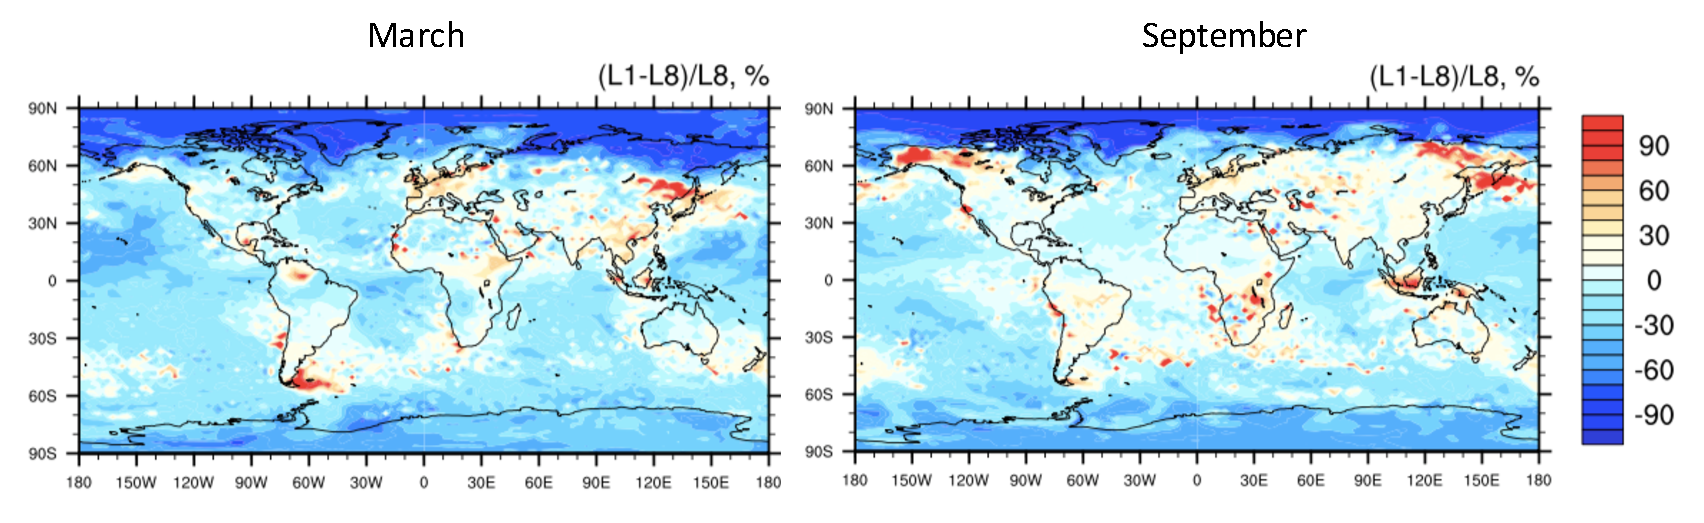
\includegraphics[width = 1\textwidth]{Figure17}
				\caption[]{\label{fig_P17} Horizontal plots pf the relative differences in BC wet deposition flux with different aging criterion (L1 v.s. L8) for March (left) and September (right).}
			\end{center}
		\end{figure}
		
		
		\begin{figure}[h] 
			\begin{center}
				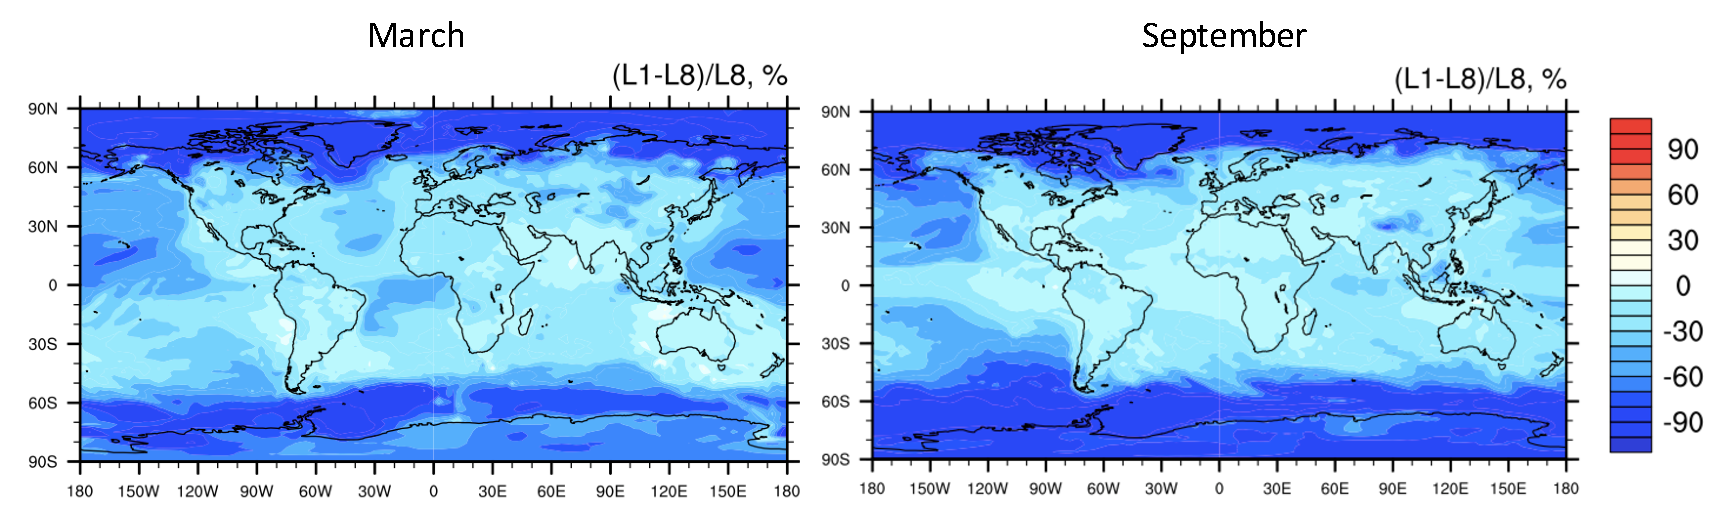
\includegraphics[width = 1\textwidth]{Figure18}
				\caption[]{\label{fig_P18} Horizontal plots pf the relative differences in BC dry deposition flux with different aging criterion (L1 v.s. L8) for March (left) and September (right).}
			\end{center}
		\end{figure}
	
	As is expected, the wet deposition rates with a smaller threshold of coating thickness giving to faster aging rates are higher in the main source regions (South East Asia, Europe, South America, Aftica, etc.) by a factor of 0.3--0.6. The wet deposition rates in case L1 become smaller than case L8 in far regions such as the distant oceans and polar regions, with the highest relative differences attaining 90~$\%$ in the Arctic. Basically this is because BC stays longer in the primary carbon mode with a larger number of monolayer criterion, and hence can be transport to distant regions. We also noticed the high values at the north edge of mainland Russia or at the south edge of South America continent, primarily because of the small values of the background concentrations (the denominator of the relative difference equation) and thus are not much concerned in our study.
	
	The dry deposition rates are positively related to the overall number concentration of BC aerosols (Figure~\ref{fig_P21}), where higher concentrations lead to faster dry scavenging. So similarly to our analysis in section~\ref{sec_1}, BC concentrations in L1 case are lower than L8 case throughout the globe, and the relative differences increase along the pathway of BC as it is transported away from the source regions. The wet scavenging rates is most sensitive to the choices of aging criterion in the high-latitude regions, with maximum differences of 99$\%$ in the Arctic for September.  
	
	\begin{figure}[h] 
		\begin{center}
			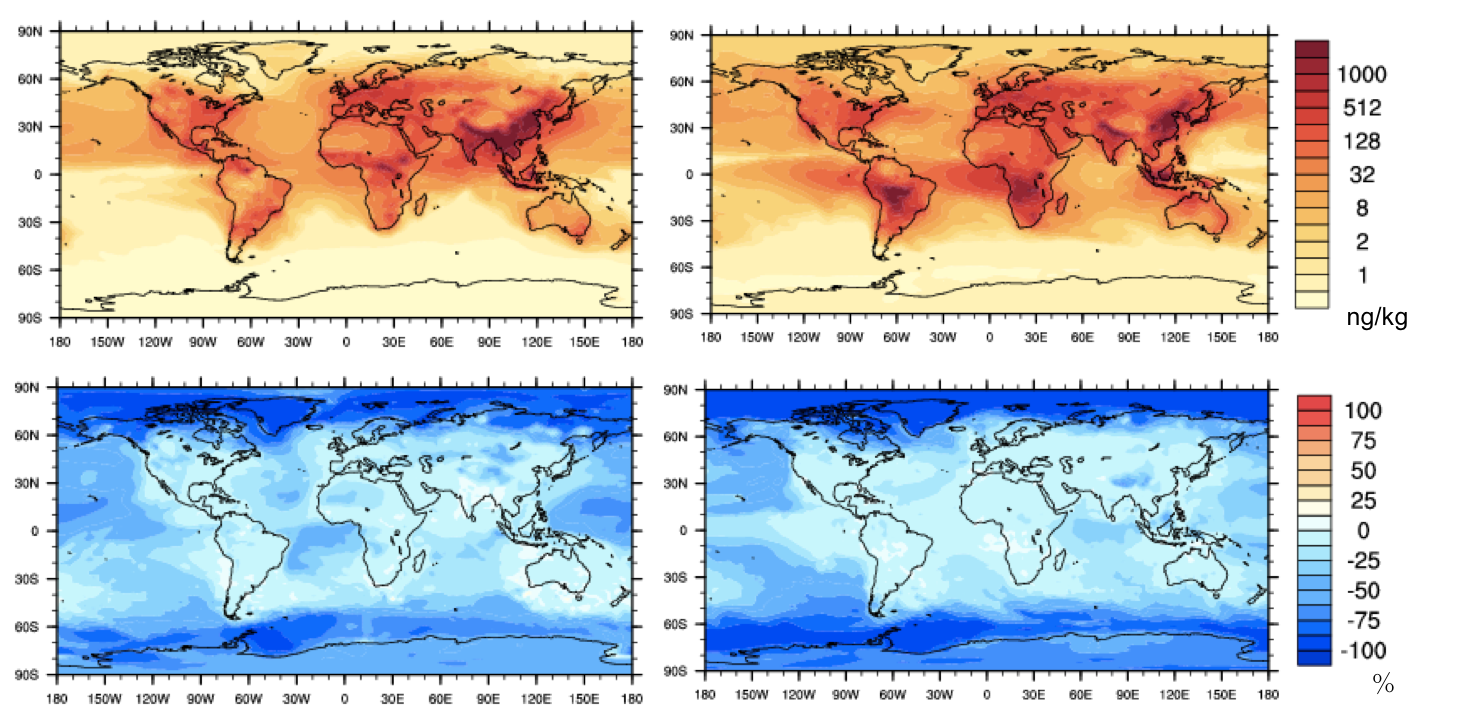
\includegraphics[width = 1\textwidth]{Figure21}
			\caption[]{\label{fig_P21} Horizontal plots of BC concentrations near the surface for different seasons (March and September).}
		\end{center}
	\end{figure}
	
	
	\subsubsection{Monolayer Effect on Radiative Forcing }
	We looked into the sensitivity of BC radiative forcing to the aging criterions, and compared their differences between L1 and L8. Figure~\ref{fig_P22} and \ref{fig_P23} shows the horizontal plots and polar plots of the annually averaged direct radiative forcing of black carbon aerosols respectively, and compares the differences between 1 monolayer and 8 monolayer as its condensation criterion. 
	\begin{figure}[H] 
		\begin{center}
			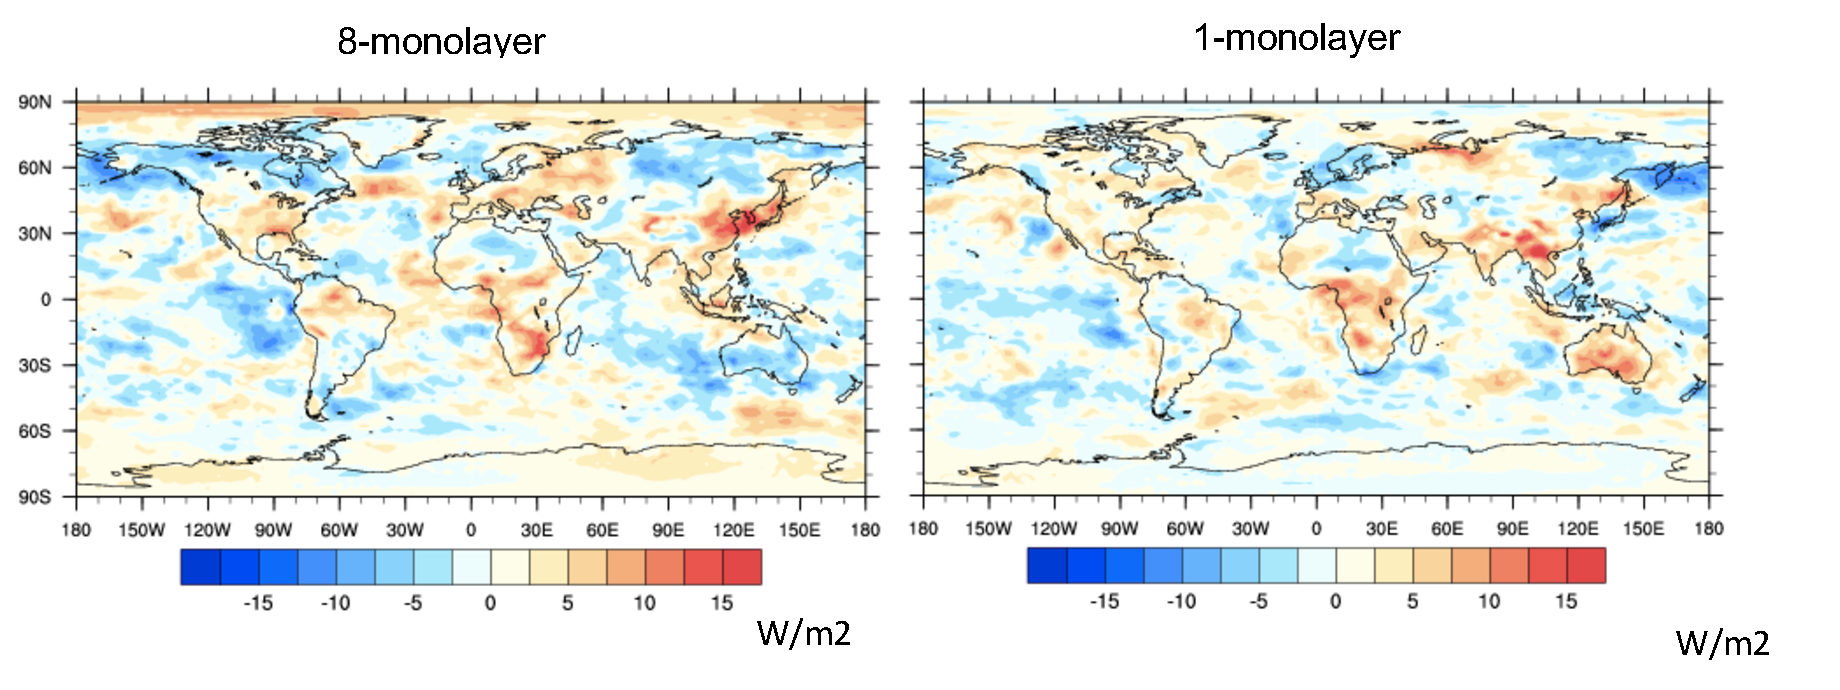
\includegraphics[width = 1\textwidth]{Figure23}
			\caption[]{\label{fig_P23} Horizontal plots of the direct radiative forcing of BC aerosols with different aging criterion (L1 v.s. L8) near the surface (992hPa).}
		\end{center}
	\end{figure}
	
	\begin{figure}[H] 
		\begin{center}
			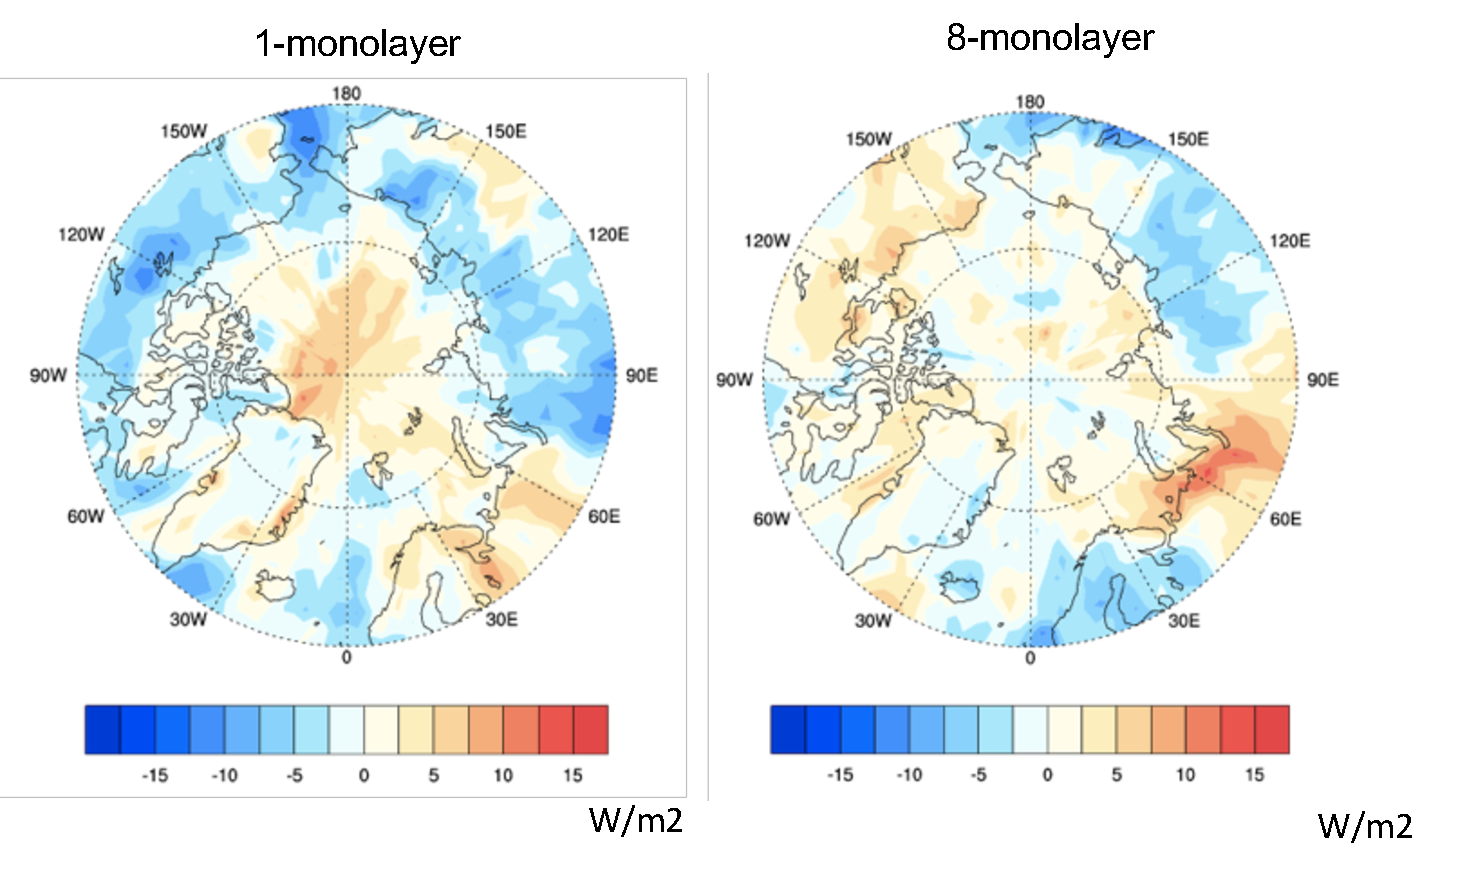
\includegraphics[width = 0.9\textwidth]{Figure22}
			\caption[]{\label{fig_P22} Polar plots of the direct radiative forcing of BC aerosols with different aging criterion (L1 v.s. L8) near the surface (992hPa).}
		\end{center}
	\end{figure}
	A smaller threshold of coating thickness gives rise to faster aging rates and a larger portion BC in the accumulation mode (internally mixed). The accumulation mode aerosols are subject to wet scavenging and removed as they are transported to distant regions. We have shown in the previous sections that generally BC mixing ratios in the L1 case are lower than L8 case throughout the globe, and the simulated BC burden is most sensitive to the choices of its aging criterion at high latitudes where the background concentrations are low. Consequently, the magnitude of the spatially averaged radiative forcing is 0.18~W$\dot{\text{m}^2}$ in the L8 case, lower than the radiative forcing of 0.48~W$\dot{\text{m}^2}$ in the L1 case because less BC are there with larger number of monolayers, and consequently faster aging and wet deposition. The magnitudes are higher in the main source regions (South East Asia, Europe, South America, Aftica, etc.) with a maximum of around 15~W$\dot{\text{m}^2}$ in both cases. 
	


	
	
	\subsubsection{BC Mass Fraction Activated by Coating Material}
	CAM-chem MAM4 assumes that the hydrophobic BC particles in  primary carbon mode will be activated and transfered to the accumulation mode after condensing a certain number of sulfate molecular layers, and it uses 8-monolayer as default. The size and hygroscopicity of BC aerosols will be increased as more condensible material is coated onto their surface, and this will lead to a decreasing supersaturation ratio to activate the particles. In MAM4, more coating material is required to age BC for larger number of monolayers, so the critical supersaturation ratio will be decreases for a larger number of monolayers. Liu et al. (2012) has estimated the critical supersaturation for 3 and 8 monolayers of sulfate to produce CCN from BC aerosols, and the values are 0.49$\%$ and 0.32$\%$ respectively. 
	
	Following Liu at al. (2012), we derived similar results and the values are 0.43$\%$ and 0.28$\%$ for 3 and 8 monolayers respectively. Furthermore, we computed the fraction of BC mass that can be activated at a certain specific supersaturation ratio based on Kohler Equation. In our estimation, we assume that BC cores follow a lognormal size distribution with a fixed standard deviation ($\sigma$=1.4) and a changeable mean diameter ranging from 80 to 150~nm considering the fact that the volume mean size for BC and POM emissions is 134~nm. The number of monolayers ranges from 1 to 23 to cover a wide range of choices. The hygroscopicity value for sulfate is 0.65, and the thickness of one sulfate monolayer is $4.76 \times 10^{-10}$~m. Figure~\ref{fig_P10} shows the results at supersaturation ratios of 0.3~$\%$ and 0.6~$\%$ since those values are typical for stratiform cloud. For a 134~nm diameter non-hygroscopic particle, the 8 monolayers of sulfate activates 65.9~$\%$ and 99.5$\%$ of BC mass with critical supersaturations of 0.3~$\%$ and 0.6~$\%$ respectively.  
	
	\begin{figure}[H] 
		\begin{center}
			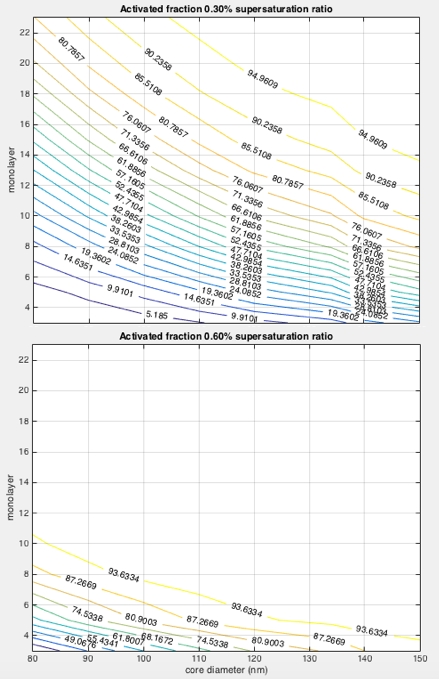
\includegraphics[width = 0.6\textwidth]{Figure10}
			\caption[]{\label{fig_P10} Fraction of BC mass that is activated at 0.3$\%$ (top) and 0.6$\%$ (bottom) supersaturation ratio.}
		\end{center}
	\end{figure}

	\subsection{BC Mixing States}
	 Figure~\ref{fig_P19} shows the comparison of BC mixing states between two MAM4 experiments, represented by the fraction of BC mixing ratio in the accumulation mode. We noticed that the model in the L1 experiment has more than 90~$\%$ of its BC mass in the accumulation mode almost everywhere throughout the globe, whereas in the L8 experiment, a decreasing trend in that fraction with increasing latitudes is obvious. The fraction is even less than 10~$\%$ for some regions in the Arctic (Greenland, Barents sea, etc.). 
	 
	 We have found that the BC mixing ratios in the L1 case are lower than the L8 case throughout the globe, and the simulated BC burden is most sensitive to the choices of its aging criterion at high latitudes. This is consistent with our results that the mixing level is more sensitive to the aging criterion at high latitudes. Comparing L8 to the L1 case, the high fraction of BC in the primary carbon mode at high latitudes seems a bit confusing because we expect BC to be more internally mixed as it is transported to distant regions. Actually it can be easily understood because less BC is aged in L8 case, so relatively a larger portion of BC in the L8 accumulation mode is deposited during its transport and little is left in the accumulation mode when the population arrives the Arctic. The spatial sensitivity of BC mixing level to latitudes is more intense in September, considering there is stronger seasonal precipitation in NH Summer (e.g., monsoon season). 
	 
	 Most of BC is in primary carbon mode are externally mixed in the Arctic that should be of our interest, considering the fact that BC has a strong climate effect in the Arctic, and its mixing states will affect its climate forcing properties such as CCN properties and optical depth properties. In the next section, we will also discuss whether the SP2 observed BC can be representative of the total BC especially in the Arctic region. We will show that most of BC detected by SP2 measurements is also externally mixed in the Arctic, and SP2 can capture most of BC in accumulation mode (internally mixed) when it is close to the source regions.

	\begin{figure}[H] 
		\begin{center}
			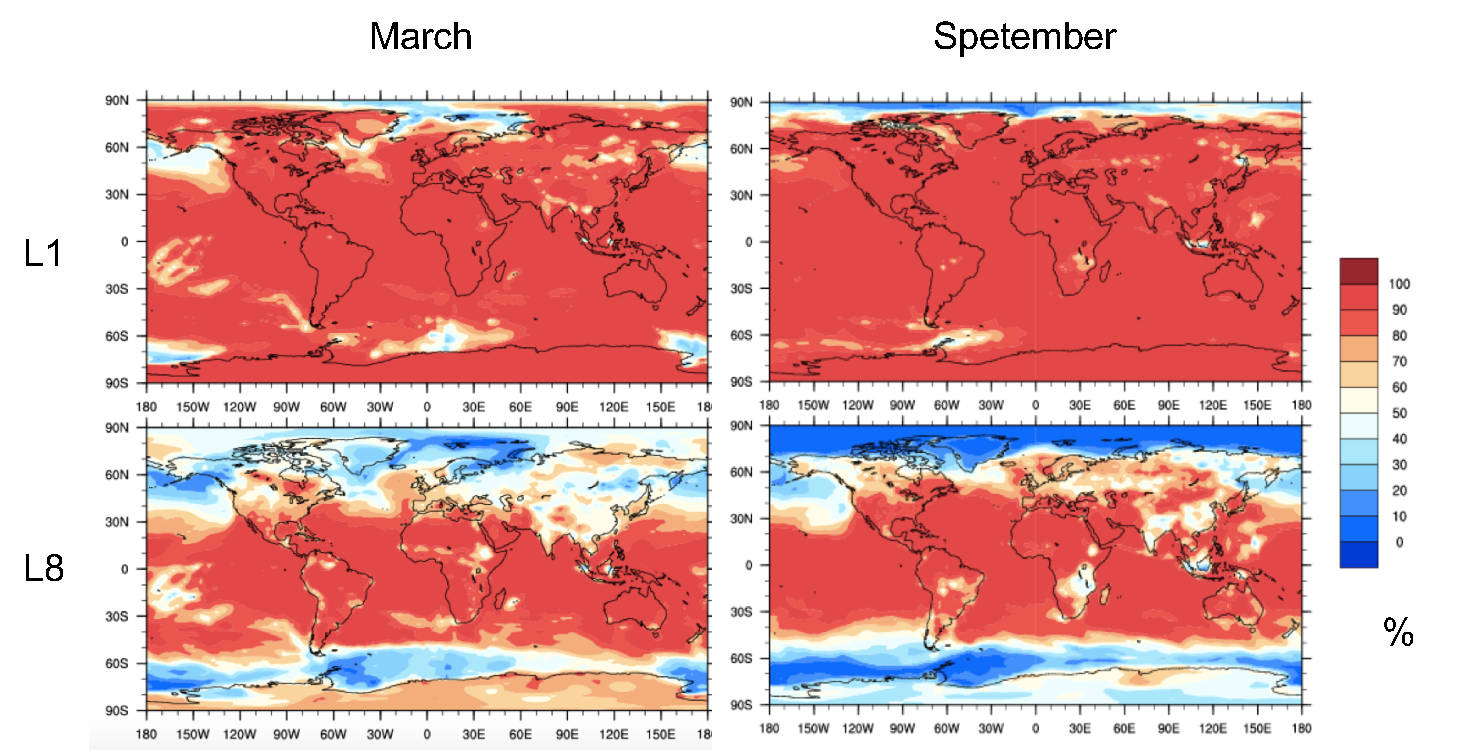
\includegraphics[width = 1\textwidth]{Figure19}
			\caption[]{\label{fig_P19} Fraction of BC mixing ratio in the accumulation mode to total BC mixing ratio (in $\%$) for L1 case (top panels) and L8 case (bottom panels) in March (left panels) and September (right panels).}
		\end{center}
	\end{figure}

	\subsection{Mass Fraction and Mixing States Observed by SP2 measurement}
	The SP2 instrument measures the BC particle cores over a calibrated volume equivalent diameter (VED) range of 55--400~nm, which is unlikely to represent the total
	ambient number and mass concentrations of BC particles \citep{Reddington2013}. In order to compare CAMChem model simulated BC with observations, we estimated the mass fraction of modeled BC in the size range corresponding to SP2 measurement. SP2 number-detection efficiency at sea level pressure is reported to be 100$\%$ for BC above 90~nm VED \citep{Schwarz2010a}, so following Reddington et al., 2013, we use 90~nm--400~nm as the efficient diameter range of SP2 measurement in this study.
	
	\subsubsection{BC Core Diameter} 
	A 4-mode version of the modal aerosol model (MAM4) is applied in
	CAMChem1.2.2. BC is emitted to the primary carbon mode, and then is
	transferred to the accumulation mode by condensation of
	$\rm{H_2SO_4}$, $\rm{NH_3}$ and $\rm{SOA}$ and by coagulation \citep{Liu2012}. In primary carbon mode, particles consist of externally
	mixed BC and OC, whereas in accumulation mode, particles consist of
	internally mixed BC and non-BC material. The version of 4 lognormal modes (MAM4) assumes that the particle size distributions in each mode has a fixed geometric standard deviation and a changeable geometric mean diameter.
	
	
	The geometric mean diameter of BC core is interpreted as:
	\begin{align*}
	d = (d_{\text{mixed}}^3 \times f_{\text{BC}})^\frac{1}{3}, 
	\end{align*}
	where $d$ is the geometric mean diameter of BC core,
	$d_{\text{mixed}}$ is the geometric mean diameter of internally mixed particles
	(\textbf{extracted from model}), and $f_{\text{BC}}$ is the volume
	fraction of BC in accumulation mode. For the following estimation of volume fraction within SP2 measurement size range, we refer to the geometric mean diameter of BC particles as its core diameter.
	
	\subsubsection{Volume Fraction Within the Size Range of SP2 Measurement}
	The CDF of lognormal number distribution of the BC cores in the diameter range between $d_{1}$ and
	$d_{2}$ is:
	\begin{align*}
	N(d_{1}, d_{2}) = \frac{1}{\text{ln}\sigma_{\text{g}}\sqrt{2\pi}}\int_{d_{1}}^{d_{2}}e^-\frac{(\text{ln}d - \text{ln}d_{\rm g})^2}{2\text{ln}^2\sigma_{\text{g}}}\text{d}(\text{ln}d),
	\end{align*}
	where $d_{\rm g}$ is the geometric mean diameter of the BC core distribution (extracted from the model, varying temporally and spatially). 
	
	The third moment of the lognormal distribution of BC core between 90 and 400~nm (proportional to the volume of BC cores whose diameter is within that size range) is:
	\begin{align*}
	V(d_{1}, d_{2}) &= \frac{1}{\text{ln}\sigma_{\text{g}}\sqrt{2\pi}}\int_{d_{1}}^{d_{2}}d^3e^-\frac{(\text{ln}d - \text{ln}d_{\rm g})^2}{2\text{ln}^2\sigma_{\text{g}}}\text{d}(\text{ln}d)  \\
	&=\frac{e^{\frac{k^2}{2}\text{ln}^2\sigma_{\rm g}+k\text{ln}d_{\rm g}}}{\text{ln}\sigma_{\text{g}}\sqrt{2\pi}}\int_{d_{1}}^{d_{2}}d^3e^-\frac{(\text{ln}d - \text{ln}d_{\text{gv}})^2}{2\text{ln}^2\sigma_{\text{g}}}\text{d}(\text{ln}d),
	\end{align*}
	where the geometric mean diameter of BC volume is represented as $\text{ln}d_{\text{gv}}
	= \text{ln}d_{\text{g}} + 3\text{ln}\sigma_{\text{g}}$
	
	So the mass fraction of the BC cores in the size range between $d_{1}$ and $d_{2}$ (in each mode) is derived as:
	
	\begin{align*}
	F(d_{1}, d_{2}) &= \frac{\frac{1}{\text{ln}\sigma_{\text{g}}\sqrt{2\pi}}\int_{d_{1}}^{d_{2}}d^3e^-\frac{(\text{ln}d - \text{ln}d_{\rm g})^2}{2\text{ln}^2\sigma_{\text{g}}}\text{d}(\text{ln}d)}
	{\frac{1}{\text{ln}\sigma_{\text{g}}\sqrt{2\pi}}\int_{-\infty}^{+\infty}d^3e^-\frac{(\text{ln}d - \text{ln}d_{\rm g})^2}{2\text{ln}^2\sigma_{\text{g}}}\text{d}(\text{ln}d)}  \\
	&=\frac{\frac{e^{\frac{k^2}{2}ln^2\sigma_{\rm g}+k\text{ln}d_{\rm g}}}{\text{ln}\sigma_{\text{g}}\sqrt{2\pi}}\int_{d_{1}}^{d_{2}}e^-\frac{(\text{ln}d - \text{ln}d_{\text{gv}})^2}{2\text{ln}^2\sigma_{\text{g}}}\text{d}(\text{ln}d)}{\frac{e^{\frac{k^2}{2}ln^2\sigma_{\rm g}+k\text{ln}d_{\rm g}}}{\text{ln}\sigma_{\text{g}}\sqrt{2\pi}}\int_{-\infty}^{+\infty}e^-\frac{(\text{ln}d - \text{ln}d_{\text{gv}})^2}{2\text{ln}^2\sigma_{\text{g}}}\text{d}(\text{ln}d)}\\
	&=\frac{1}{\text{ln}\sigma_{\text{g}}\sqrt{2\pi}}\int_{d_{1}}^{d_{2}}e^-\frac{(\text{ln}d - \text{ln}d_{\text{gv}})^2}{2\text{ln}^2\sigma_{\text{g}}}\text{d}(\text{ln}d) \\
	&=\frac{1}{2}[\text{erf}(\frac{\text{ln}d_{2} - \text{ln}d_{\text{gv}}}{\sqrt{2}\text{ln}\sigma_{\rm g}})-\text{erf}(\frac{\text{ln}d_{1} - \text{ln}d_{\text{gv}}}{\sqrt{2}\text{ln}\sigma_{\rm g}})],
	\end{align*}
	
	The above mass fraction for primary carbon mode ($F_{\text{pc}}(d_{1}, d_{2})$) and for accumulation mode ($F_{\text{accu}}(d_{1}, d_{2}$) do not add up to 1:
	\[F_{\text{accu}}(d_{1}, d_{2}) + F_{\text{pc}}(d_{1}, d_{2}) \neq 1,\]
	
	
	
	\textbf{Within the size range (90--400~nm)}, the ratios of the mass of BC cores in each mode to the total mass of BC cores are computed as:
	\begin{align*}
	f_{\text{accu}} = \frac{F_{\text{accu}}(d_{1}, d_{2})M_{\text{accu}}}{F_{\text{accu}}(\text{d}_{1}, d_{2})M_{\text{accu}}+F_{\text{pc}}(d_{1}, d_{2})M_{\text{pc}}}\\
	f_{\text{pc}} = \frac{F_{\text{pc}}(d_{1}, d_{2})M_{\text{pc}}}{F_{\text{accu}}(d_{1}, d_{2})M_{\text{accu}}+F_{\text{pc}}(d_{1}, d_{2})M_{\text{pc}}}
	\end{align*}
	\[f_{\text{accu}} + f_{\text{pc}} = 1,\]
	
	where $f_{\text{accu}}$ is the mass fraction of BC cores in
	accumulation mode, $f_{\text{pc}}$ is the mass fraction of BC cores in
	primary carbon mode, $M_{\text{accu}}$ and $M_{\text{pc}}$ are the mass mixing ratio of BC cores
	in accumulation mode and primary carbon mode, respectively.
	
	Sketch of F and f are shown in Figure~\ref{fig_R1}, Figure~\ref{fig_R2} and Figure~\ref{fig_R3}.
	
	\begin{figure}[H] 
		\begin{center}
			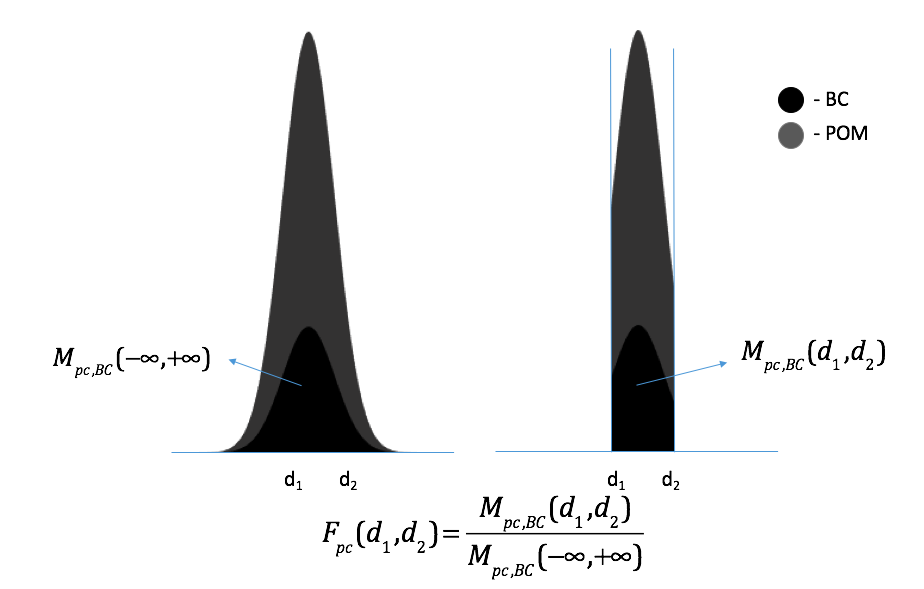
\includegraphics[width = 0.8\textwidth]{Rplot05}
			\caption[]{\label{fig_R1} BC mass fraction within the SP2 size range for primary carbon mode $F_{\text{pc}}(d_{1}, d_{2})$.}
		\end{center}
	\end{figure}
	
	\begin{figure}[H] 
		\begin{center}
			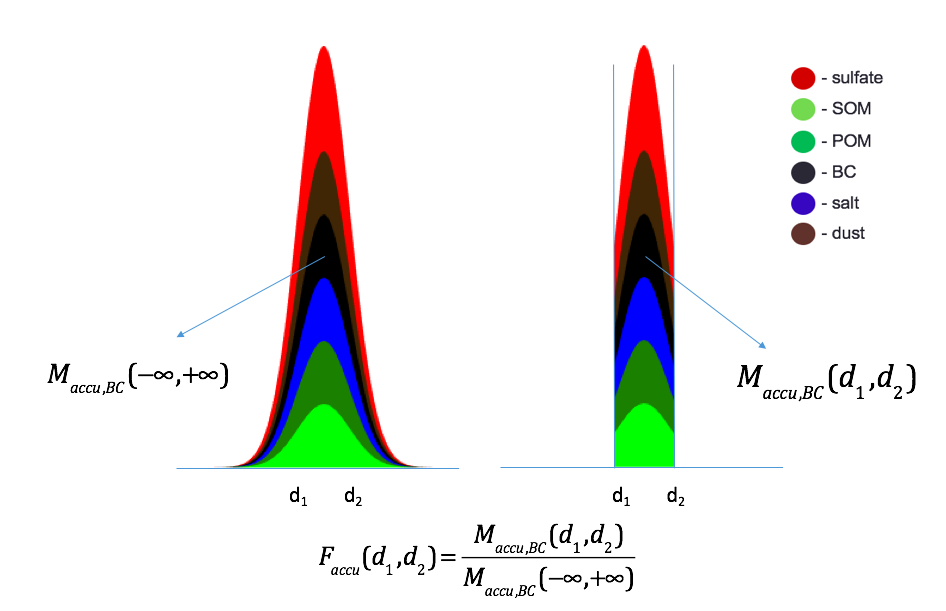
\includegraphics[width = 0.8\textwidth]{Rplot06}
			\caption[]{\label{fig_R2} BC mass fraction within the SP2 size range for accumulation mode $F_{\text{accu}}(d_{1}, d_{2})$.}
		\end{center}
	\end{figure}
	
	\begin{figure}[H] 
		\begin{center}
			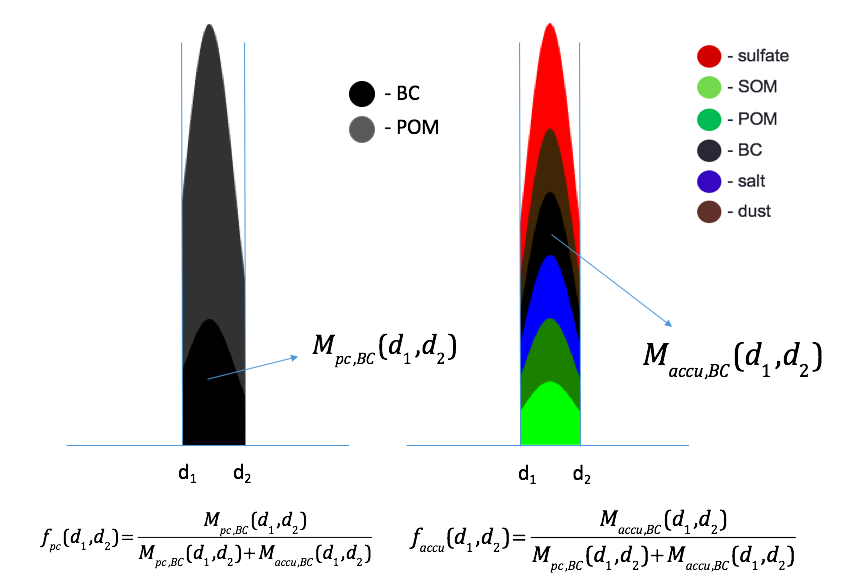
\includegraphics[width = 0.7\textwidth]{Rplot07}
			\caption[]{\label{fig_R3} The ratios of BC mass in the SP2 size range in each mode to the total BC mass in the SP2 size range, for primary carbon mode $f_{\text{pc}}(d_{1}, d_{2})$ and for accumulation mode $f_{\text{accu}}(d_{1}, d_{2})$.}
		\end{center}
	\end{figure}
	
	
	Generally, the mixing ratio of BC particles in the accumulation mode is higher ($M_{\text{accu}}$) than that in the primary carbon mode ($M_{\text{pc}}$) when it is distant from the source regions (e.g., Indian Ocean, Atlantic Ocean) (Figure~\ref{fig_R4}), primarily because black carbon will be transfered from the fresh, hydrophobic mode (primary carbon) into the aged, hydrophilic mode (accumulation) during transportation. We also observe that for some Arctic regions (e.g., Greenland), however, BC mixing ratio can be higher in the primary carbon mode than in the accumulation mode.
	
	BC mass fractions within the SP2 size range ($F_{\text{pc}}(90~\text{nm}, 400~\text{nm})$ and
	$F_{\text{accu}}(90~\rm nm, 400~\rm nm)$) are shown in Figure~\ref{fig_R5}. For primary carbon mode
	(upper panel), SP2 would be able to detect most of BC ($\textgreater$60$\%$) over the ocean and throughout the North Pole, and less of BC ($\textless$40$\%$) in regions like central Africa, Northeast Asia and Australia. For accumulation mode (lower panel), this portion is higher when it is close to the sources (e.g., South East Asia, Europe), and lower at high latitudes. We also observe that the distributions of the above mass fractions (Figure~\ref{fig_R5}) have similar pattern with the size distributions of BC cores (Figure~\ref{fig_R6}), which indicates that the low values of the mass fraction ($F_{\text{pc}}(90~\text{nm}, 400~\text{nm})$ and $F_{\text{accu}}(90~\text{nm}, 400~\text{nm}$) are highly due to the small geometric mean diameter of BC cores ($\textless$90~nm)in that region.
	\begin{figure}[H] 
		\begin{center}
			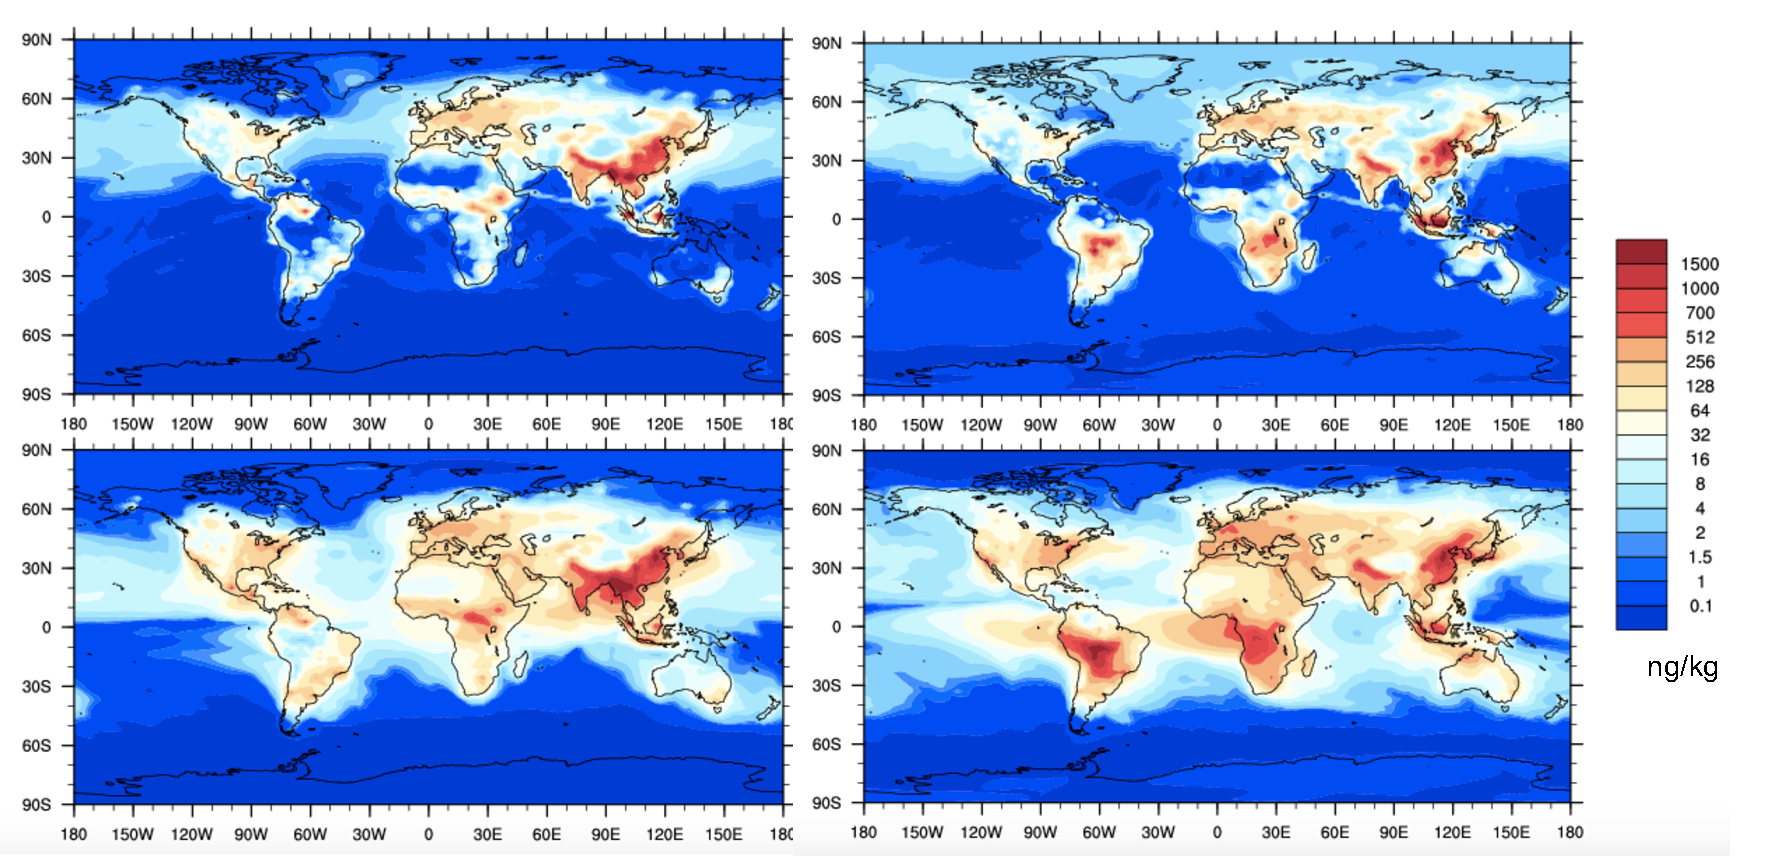
\includegraphics[width = 1\textwidth]{Rplot01}
			\caption[]{\label{fig_R4}BC mass mixing ratio ($M_{\rm pc}$ and $M_{\rm accu}$) in primary carbon mode (top) and in accumulation mode (bottom), for surface layer, March and September.}
		\end{center}
	\end{figure}
	
	\begin{figure}[H] 
		\begin{center}
			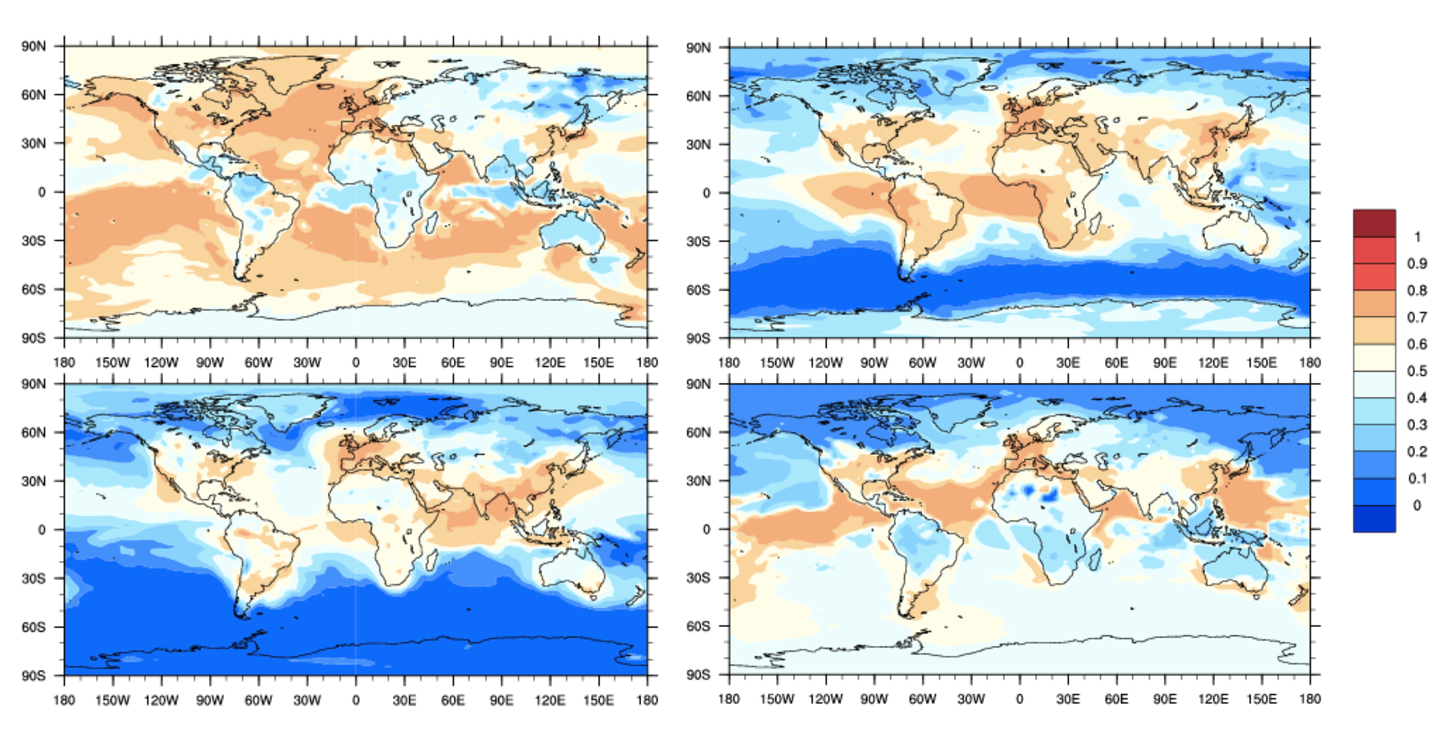
\includegraphics[width = 0.9\textwidth]{Rplot02}
			\caption[]{\label{fig_R5} BC mass fraction between 90 and 400~nm ($F_{\rm pc}$ and $F_{\rm accu}$) in the primary carbon mode (top) and accumulation mode (bottom), for surface layer, in March and September.}
		\end{center}
	\end{figure}
	
	\begin{figure}[H] 
		\begin{center}
			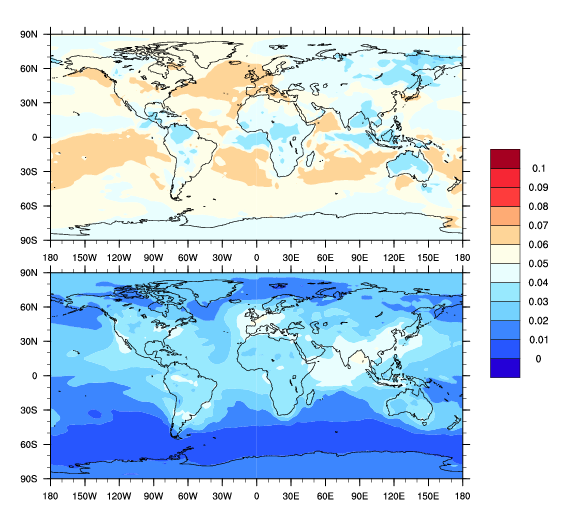
\includegraphics[width = 0.9\textwidth]{Rplot03}
			\caption[]{\label{fig_R6} Geometric mean diameter of BC core ($\mu$m) in primary carbon mode (top) and accumulation mode (bottom), for surface layer, in March and September.}
		\end{center}
	\end{figure}
	
	
	
	The ratios of BC mixing ratio in each mode within the SP2 size range to the total BC mixing ratio within the SP2 size range ($f_{\rm pc}$ and $f_{\rm accu}$) are shown in Figure~\ref{fig_R7}, which represents the mixing states of BC particles that are captured by SP2 measurements. Most of them are internally mixed in the low and middle
	latitudes ($f_{\rm accu}\textgreater$60$\%$), and are externally mixed at high latitudes ($f_{\rm pc}\textgreater$60$\%$). The mixing state can vary spatially in the Arctic region,
	which should be taken into consideration when comparing modeled BC
	with SP2 measurements. Fractions in two panels should add up to 1.
	
	
	
	\begin{figure}[H] 
		\begin{center}
			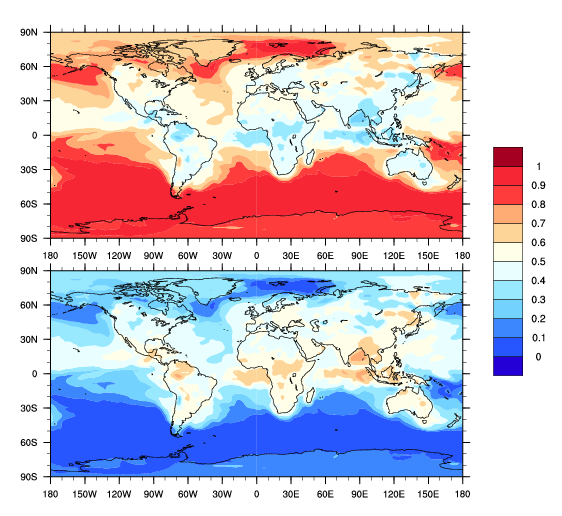
\includegraphics[width = 0.9\textwidth]{Rplot04}
			\caption[]{\label{fig_R7} Ratio of BC mixing ratio within SP2 size range to total BC mixing ratio within SP2 size range in primary carbon mode $f_{\rm pc}$ (top) and in accumulation mode $f_{\rm accu}$ (bottom), for surface layer, in March and September.}
		\end{center}
	\end{figure}
	
	
	\newpage
	\subsection{Process Analysis of BC Aging}
	Fierce et al (2016) has derived an parameterized e-folding time $\tau_{\rm overall}$ from the approximate range of condensation growth rate and number concentration for specific locations (Equation~\ref{eq_1}). 
	\begin{align}{\label{eq_1}}
	\tau_{\rm overall} \approx (k_{\rm cond}I_{\rm cond} + k_{\rm coag}N)^{-1}
	\end{align}, where $I_{\rm cond}$ is the condensation growth rate (in nm/h) and $N$ is the overall number concentration of aerosol particles. This parameterization can be used an a reference for global models. 
	\subsubsection{BC Condensation Growth Rate from CAM-chem}		
	In our study, we derived the condensation growth rate $I_{\rm cond}$ as the volume condensation rate over the total aerosol surface area. As is mentioned in 3.2, the condensation of SOA is reversible, so the total condensation rate can be positive or negative. Since all fresh BC particles are in the primary carbon mode, we computed the condensation growth rate using the volume condensation rate and surface area extracted from the primary carbon mode. The PartMC-MOSAIC parameterized aging timescales can then be represented as:
		\begin{figure}[H] 
			\begin{center}
				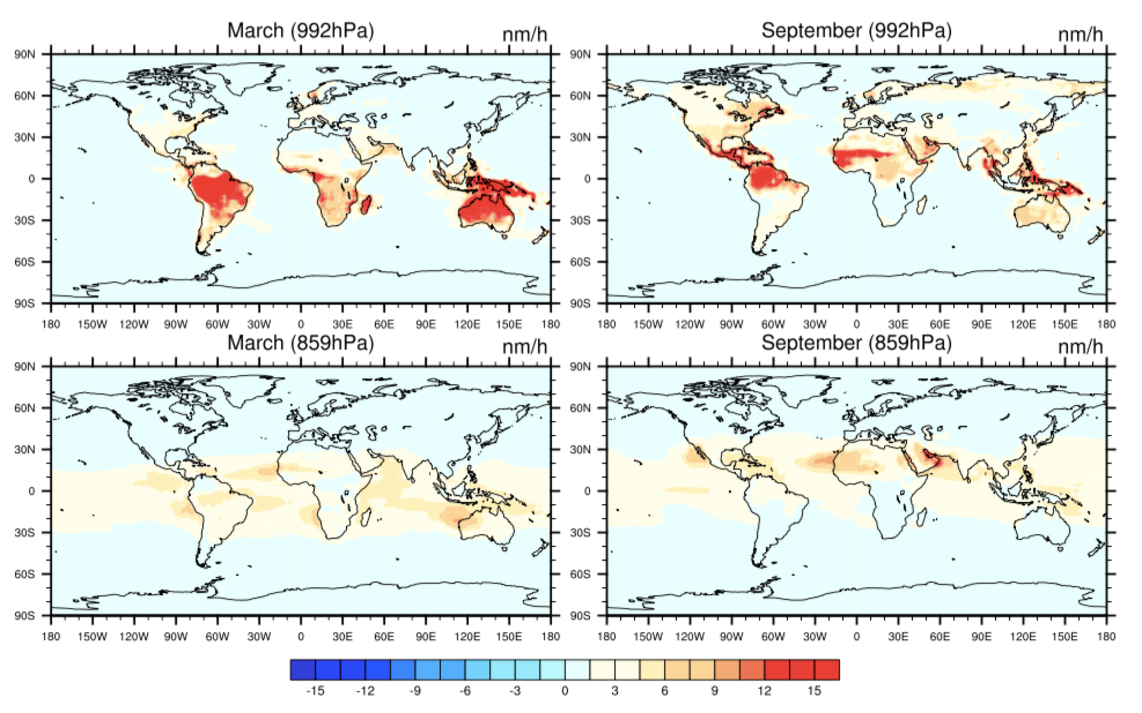
\includegraphics[width = 0.9\textwidth]{Figure24}
				\caption[]{\label{fig_p24} Geometric mean diameter of BC core ($\mu$m) in primary carbon mode (top) and accumulation mode (bottom), for surface layer, in March and September.}
			\end{center}
		\end{figure}
	\subsubsection{BC Condensation Growth Rate from Experiment}
	
	
	
	


	\section{Summary and Conclusion}
	
	\section{Appendix}
	
	\subsection{Configuration of CAM-chem Model}
	Create a directory for the code, download the code, go into the scripts directory in the source code:
	\begin{lstlisting}[xleftmargin=0.01\textwidth, xrightmargin=0.01\textwidth]
	mkdir ~/cesm1_2_2_CAMChem
	cd /glade/u/home/yinruili/cesm1_2_2_CAMChem/script
	\end{lstlisting}
	
	Create a new case:
	\begin{lstlisting}[xleftmargin=0.01\textwidth, xrightmargin=0.01\textwidth]
	setenv CCSMTAG	cesm1_2_2_CAMChem
	setenv CASE	FSTRATMAM4_extract_offmeteo_5
	setenv MACH      yellowstone
	setenv CCSMROOT  /glade/u/home/yinruili/${CCSMTAG}
	setenv CASEROOT  /glade/scratch/yinruili/cases/$CASE
	# create a new case using MAM4 and free-running
	./create_newcase -case $CASEROOT -mach $MACH -res  f19_f19 -compset FSTRATMAM4
	# create a new case using MAM4 with offline-meteorology
	./create_newcase -case $CASEROOT -mach $MACH -res  f19_f19 -user_compset GEOS_CAM5%SMA4_CLM40%SP_CICE%PRES_DOCN%DOM_RTM_SGLC_SWAV 
	\end{lstlisting}
	
	Edit runtime options using xmlchange: env$\_$run.xml
	\begin{lstlisting}[xleftmargin=0.01\textwidth, xrightmargin=0.01\textwidth]
	#e.g., start at 2010-01-01, run for 12 months.
	./xmlchange  -file env_run.xml -id  STOP_N        -val '12'
	./xmlchange  -file env_run.xml -id  STOP_OPTION   -val 'nmonth'
	./xmlchange  -file env_run.xml -id  RUN_STARTDATE -val '2010-01-01'
	\end{lstlisting}
	Edit namelist: user\_nl\_cam (This file will be created after you set up the case (./cesm\_setup), but it can also be created manually (using cat) before that. I would prefer the latter option).
	\begin{lstlisting}[xleftmargin=0.01\textwidth, xrightmargin=0.01\textwidth]
	#add variables that you would like to see in the output
	cat <<EOF >! user_nl_cam
	history_aerosol     = .true.
	history_amwg        = .true.
	history_aero_optics = .true.
	mfilt           = 1,  1,
	# nhtfrq = 0, the file will be monthly average
	# nhtfrq = -24, the frequency is input as 24 hours (daily)
	nhtfrq          = 0,  -24,
	# avgflag_pertape = 'A', averaged data
	# avgflag_pertape = 'I', instantaneous data
	avgflag_pertape ='A','A',
	# variables you would like to add into monthly file (fincl1) and hourly file (fincl2)
	fincl1          ="bcgascon","bcagingcon","bcmasscon","surface","volumn","bcagingcoag","bcmasscoag","numa1","numa2","numa3","numa4", "dgnd_a01", "dgnd_a02", "dgnd_a03", "dgnd_a04", "dgnw_a01", "dgnw_a02","dgnw_a03","dgnw_a04","dgnumwet1","dgnumwet2","dgnumwet3","dgnumwet4"
	fincl2          ="bcgascon","bcagingcon","bcmasscon","surface","volumn","bcagingcoag","bcmasscoag","numa1","numa2","numa3","numa4", "dgnd_a01", "dgnd_a02", "dgnd_a03", "dgnd_a04", "dgnw_a01", "dgnw_a02","dgnw_a03","dgnw_a04","dgnumwet1","dgnumwet2","dgnumwet3","dgnumwet4"
	\end{lstlisting}
	
	Set offline meteorology:
	\begin{lstlisting}[xleftmargin=0.01\textwidth, xrightmargin=0.01\textwidth]
	inithist = 'MONTHLY'
	ncdata        = '/glade/p/cesm/cseg//inputdata/atm/cam/inic/fv/camchem_ic_2008-01-01_1.9x2.5_L56_c110118.nc'
	bnd_topo  = '/glade/p/cesm/cseg/inputdata/atm/cam/met/USGS-gtopo30_1.9x2.5_phys_geos5_c100929.nc'
	met_data_file   = '2010/GEOS5.2_19x2_20100101.nc'
	met_data_path   = '/glade/p/cesmdata/cseg/inputdata/atm/cam/met/GEOS5'
	met_filenames_list      = '/glade/p/cesmdata/cseg/inputdata/atm/cam/met/GEOS5/GEOS5_filenames_list_c120516.txt'
	met_max_rlx     = 0.10
	met_qflx_factor = 0.84
	\end{lstlisting}
	
	Configure the model:
	\begin{lstlisting}[xleftmargin=0.01\textwidth, xrightmargin=0.01\textwidth]
	./cesm_setup
	\end{lstlisting}
	
	Modify the source code and add them into ./SourceMode
	\begin{lstlisting}[xleftmargin=0.01\textwidth, xrightmargin=0.01\textwidth]
	# For example, I modified two files (al_aero_gasaerexch_sens_icon.F90 and modal_aero_coag.F90), and copied them into the SourceMode directory so that the model can be build with the modified code. 
	cp /glade/u/home/yinruili/cesm1_2_2_CAMChem/scripts/sourcemode/modal_aero_gasaerexch.F90 ./SourceMods/src.cam/modal_aero_gasaerexch.F90
	cp /glade/u/home/yinruili/cesm1_2_2_CAMChem/scripts/sourcemode/modal_aero_coag.F90 ./SourceMods/src.cam/

	\end{lstlisting}
	
	Build the model, and then go into the case root and run the model:
	\begin{lstlisting}[xleftmargin=0.01\textwidth, xrightmargin=0.01\textwidth]
	./$CASE.build
	cd $CASEROOT
	./$CASE.run
	\end{lstlisting}
	
	
	\bibliographystyle{plain-local-srefid}
	\bibliography{refs}
	
	
	
	
	
	
	%%%%%%%%%%%%%%%%%%%%%%%%%%%%%%%%%%%%%%%%%%%%%%%%%%%%%%%%%%%%%%%%%%%%%%%%%%%%%%%%
	


Bauer, S. E.,  S. Menon, D. Koch, T. C. Bond, and K. Tsigaridis. A global modeling study on carbonaceous aerosol microphysical characteristics and radiative forcing. Atmos. Chem. Phys., 10:4543–4592, 2010.

Bond, T. C., Streets, D. G., Yarber, K. F., Nelson, S. M., Woo, J. H.,and Klimont, Z.: A technology-based global inventory of black and organic carbon emissions from combustion, J. Geophys. Res.-Atmos., 109, D14203, doi:10.1029/2003jd003697, 2004.

Bond, T., Doherty, S., Fahey, D., Forster, P., Berntsen, T., DeAngelo, B., Flanner, M., Ghan, S.,Kärcher, B., and Koch, D.: Bounding the role of black carbon in the climate system: a scientific 10assessment, J. Geophys. Res.-Atmos., 118, 5380–5552, doi:10.1002/jgrd.50171, 2013.

Cooke, W. F., and J. N. Wilson. A global black carbon aerosol model. J. Geophys. Res., 101:19395–19408, 1996.
Croft, B., Lohmann, U., and von Salzen, K.: Black carbon ageing in the Canadian Centre for Climate modelling and analysis atmo- spheric general circulation model, Atmos. Chem. Phys., 5, 1931– 1949, doi:10.5194/acp-5-1931-2005, 2005. 
Liu, J. F., Fan, S. M., Horowitz, L. W., and Levy, H.: Evalua- tion of factors controlling long-range transport of black car- bon to the Arctic, J. Geophys. Res.-Atmos., 116, D04307, doi:10.1029/2010jd015145, 2011. 

Riemer, N., Vogel, H., and Vogel, B.: Soot aging time scales in polluted regions during day and night, Atmos. Chem. Phys., 4, 1885–1893, doi:10.5194/acp-4-1885-2004, 2004. 

Schwarz, J. P., Spackman, J. R., Gao, R. S., Watts, L. A., Stier, P., Schulz, M., Davis, S. M., Wofsy, S. C., and Fahey, D. W.: Global- scale black carbon profiles observed in the remote atmosphere and compared to models (vol 37, art L18812, 2010), Geophys. Res. Lett., 37, L23804, doi:10.1029/2010gl046007, 2010. 

Shindell, D. T., Chin, M., Dentener, F., Doherty, R. M., Faluvegi, G., Fiore, A. M., Hess, P., Koch, D. M., MacKenzie, I. A., Sander- son, M. G., Schultz, M. G., Schulz, M., Stevenson, D. S., Teich, H., Textor, C., Wild, O., Bergmann, D. J., Bey, I., Bian, H., Cuve- lier, C., Duncan, B. N., Folberth, G., Horowitz, L. W., Jonson, J., Kaminski, J. W., Marmer, E., Park, R., Pringle, K. J., Schroeder, S., Szopa, S., Takemura, T., Zeng, G., Keating, T. J., and Zu- ber, A.: A multi-model assessment of pollution transport to the Arctic, Atmos. Chem. Phys., 8, 5353–5372, doi:10.5194/acp-8- 5353-2008, 2008. 

Fan, S. M., Schwarz, J. P., Liu, J., Fahey, D. W., Ginoux,P., Horowitz, L. W., Levy, H., Ming, Y., and Spackman, J. R.: Inferring ice formation processes from global-scale black carbon profiles observed in the remote atmosphere and model simulations, J. Geophys. Res.-Atmos., 117, D23205, doi:10.1029/2012jd018126, 2012.

Flanner, M. G., Zender, C. S., Randerson, J. T., and Rasch, P. J.: Present-day climate forcing and response from black carbon in snow, J. Geophys. Res., 112, D11202, forssdoi:10.1029/2006JD008003, 2007.

Forsstro¨m, S., E. Isaksson, R. B. Skeie, J. Stro¨m, C. A. Pedersen, S. R. Hudson, T. K. Berntsen, H. Lihavainen, F. Godtliebsen, and S. Gerland, Elemental carbon measurements in European Arctic snow packs,J. Geophys. Res. Atmos., 118, 13,614–13,627, doi:10.1002/2013JD019886, 2013.

Hakami, A., Henze, D. K., Seinfeld, J. H., Chai, T., Tang, Y., Carmichael, G. R., and Sandu, A.: Adjoint inverse modeling of black carbon during the Asian Pacific Regional Aerosol Charac- 30 terization Experiment, J. Geophys. Res.-Atmos., 110, D14301,doi:10.1029/2004jd005671,2005.

Highwood, E. J. and Kinnersley, R. P.: When smoke gets in our eyes: The multiple impacts of atmospheric black carbon on climate, air quality and health, Environ. Int., 32, 560–566, doi:10.1016/j.envint.2005.12.003, 2006.

Huang, Y., S. Wu, M. K. Dubey, and N. H. F. French.  Impact of aging mechanism on model simulated carbonaceous aerosols. Atmos. Chem. Phys., 13: 6329-6343, 2013.

Koch, D., Schulz, M., Kinne, S., McNaughton, C., Spackman, J.R., Balkanski, Y., Bauer, S., Berntsen, T., Bond, T. C., Boucher, O., Chin, M., Clarke, A., De Luca, N., Dentener, F., Diehl, T.,Dubovik, O., Easter, R., Fahey, D. W., Feichter, J., Fillmore,D., Freitag, S., Ghan, S., Ginoux, P., Gong, S., Horowitz, L.,Iversen, T., Kirkevåg, A., Klimont, Z., Kondo, Y., Krol, M., Liu, X., Miller, R., Montanaro, V., Moteki, N., Myhre, G., Penner,J. E., Perlwitz, J., Pitari, G., Reddy, S., Sahu, L., Sakamoto, H.,Schuster, G., Schwarz, J. P., Seland, Ø., Stier, P., Takegawa, N., Takemura, T., Textor, C., van Aardenne, J. A., and Zhao, Y.: Evaluation of black carbon estimations in global aerosol models, Atmos. Chem. Phys., 9, 9001–9026, doi:10.5194/acp-9-9001-2009,2009.

Lamarque, J. F., et al. "CAM-chem: description and evaluation of interactive atmospheric chemistry in the Community Earth System Model, Geosci. Model Dev., 5, 369–411, doi: 10.5194." (2012).

Fierce, Laura, et al. "Black carbon absorption at the global scale is affected by particle-scale diversity in composition." Nature Communications 7 (2016).

Liu, X., et al. Toward a minimal representation of aerosols in climate models: description and evaluation in the Community Atmosphere Model CAM5. Geosci. Model Dev., 5, 709–739, 2012.
Liu, X., et al. "Description and evaluation of a new 4-mode version of Modal Aerosol Module (MAM4) within version 5.3 of the Community Atmosphere Model." Geoscientific Model Development Discussions 8.9 (2015).

Quaas, J., Ming, Y., Menon, S., Takemura, T., Wang, M., Penner, J. E., Gettelman, A., Lohmann, U., Bellouin, N., Boucher, O., Sayer, A. M., Thomas, G. E., McComiskey, A., Feingold, G., Hoose, C., Kristjánsson, J. E., Liu, X., Balkanski, Y., Donner, L. J., Ginoux, P. A., Stier, P., Grandey, B., Feichter, J., Sednev, I., Bauer, S. E., Koch, D., Grainger, R. G., Kirkevåg, A., Iversen, T., Seland, Ø., Easter, R., Ghan, S. J., Rasch, P. J., Morrison, H., Lamarque, J.-F., Iacono, M. J., Kinne, S., and Schulz, M.: Aerosol indirect effects – general circulation model intercomparison and evaluation with satellite data, Atmos. Chem. Phys., 9, 8697-8717, doi:10.5194/acp-9-8697-2009, 2009.

Riemer, N., M. West, R. A. Zaveri, and R. C. Easter. Estimating black carbon aging time- scales with a particle-resolved aerosol model. J. Aerosol Sci., 41(1):143–158, 2010. DOI: 10.1016/j.jaerosci.2009.08.009.
Schulz, M., Textor, C., Kinne, S., Balkanski, Y., Bauer, S., Berntsen, T., Berglen, T., Boucher, O., Dentener, F., Guibert, S., Isaksen, I. S. A., Iversen, T., Koch, D., Kirkevåg, A., Liu, X., Montanaro, V., Myhre, G., Penner, J. E., Pitari, G., Reddy, S., Seland, Ø., Stier, P., and Takemura, T.: Radiative forcing by aerosols as derived from the AeroCom present-day and pre-industrial simulations, Atmos. Chem. Phys., 6, 5225-5246, doi:10.5194/acp-6-5225-2006, 2006.

Wilson, J., C. Cuvelier, and F. Raes. A modeling study of global mixed aerosol fields. J. Geophys. Res., 106:34081–34108, 2001.

Zuberi, B., Johnson, K. S., Aleks, G. K., Molina, L. T., and Laskin, A.: Hydrophilic properties of aged soot, Geophys. Res. Lett., 32, L01807, doi:10.1029/2004gl021496, 2005.

	
\end{document}
%%%%%%%%%%%%%%%%%%%%%%%%%%%%%%%%%%%%%%%%%%%%%%%%%%%%%%%%%%%%%%%%%%%%%%%%%%%%%%%%
%%%%%%%%%%%%%%%%%%%%%%%%%%%%%%%%%%%%%%%%%%%%%%%%%%%%%%%%%%%%%%%%%%%%%%%%%%%%%%%%
